\part{Semantic Representation}
\label{part:semantic-representation}

\chapter*{Abstract}
\label{chap:semantic-representation_abstract}
% - Terrain generation usually focus on geometry processing \\
% - Some works include soil materials in their process \\
% - But no semantic information is preserved \\
% - Many fields use topologic maps to describe the environment \\
% ** see Travel books \\
% - Our method to abstract the geometry and focus on the symbolic \\
% - ... 
This chapter introduces a novel method for procedural terrain generation, which leverages a sparse representation of environmental features to produce landscapes that are lightweight, plausible and adaptable to user desires. The method differs from traditional terrain generation approaches by emphasizing multi-scale user interaction and incorporating expert knowledge to model the evolution of terrain features over time. By representing terrain features as discrete entities, or "\glosses{EnvObj}", the method enables dynamic interaction between these entities and their surrounding environment, represented through continuous scalar and vector fields. The generation process is iterative and allows for user-guided modifications at any iteration, including the introduction of environmental events that can influence the terrain's evolution. The proposed approach is particularly flexible, capable of generating both terrestrial and underwater landscapes with a focus on large-scale plausibility and detailed, localized feature representation. 


% Automated terrain generation is a key component of natural scene digital modeling for animated movies and video games. Many landscapes have been studied and are synthesised with more and more realism. 
% Different processes can be used and combined to achieve these scenes: fractal terrains \cite{Musgrave1989,Prusinkiewicz1993a}, erosion simulation \cite{Cordonnier2023, Mei2007}, manual modeling \cite{DeCarpentier, Guerin2022}, geological simulation \cite{Cortial2019,Cordonnier2017a}, ... The high quality of synthesis for such environment is due to the possibility to observe these environments from many point of views: long-distance gazing, hiking on mountains, remote sensing, aerial imaging, ... 
% Thanks to the quality of the digital modeling, the entertainment industry display often breathtaking land scenes.

% Underwater scenes are rarely created in these media for multiple reasons: these environments are not completely understood and mastered as much as land environments because they are difficult to access, we lack the capacity to see them at a larger scale (unlike mountains for example) and the underlying process that forms these landscapes are much more complex to simulate.

% These limitations cause animated movies and video games studios to avoid as much as possible underwater environments. 

% However, these environments are important for the study of biology, geology, and, by extension, robotics. Due to the complexity, limitations and danger of underwater human operations, underwater robots are more and more used for marine environment monitoring\cite{Maslin2021, Williams2016, Dunbabin2020, Palmer2021}. Yet the validation process of such underwater robot is expensive, with heavy logistic, and it is often  impossible to find the appropriated environment to test the system. Thus, underwater robotics requires simulation capacities, to be able to test the robot's algorithms in very specific environment and conditions. But for now, roboticians are lacking the capacity to test on realistic virtual scenes, and so only test them on synthetic scenarios that do not correlate with real world terrains. For that, they need to manipulate more precisely the characteristics of the underwater environment, at different scales.

% The difficulties to visualize and study the underwater environments on a large scale at the same time as a small scale is an obstacle to the procedural generation and simulation of scenes that are coherent in these two different scales. 
% A solution to this problem could be a bottom-up approach, simulating at the smallest scale the behaviour of all the elements of the environment. Computing such a simulation in order to generate an entire ecosystem is an near-impossible task due to time and memory complexity. 

% The method we propose provides a way to procedurally generate environments on multiple scales without introducing such complexity by using a sparse representation of the environment using \glosses{EnvObj}.
% The \glosses{EnvObj} only have access to local values of the environments to spawn, grow and die. The use of local interaction with environment values removes the need for complex interconnections between all elements of the terrain, providing a parallelisable generation process at large to small scales.
% Defining \glosses{EnvObj} of the terrain as parametric models based on point, curve or region skeletons provides a lightweight representation of the terrain that the user can interact with. The interaction with the simulation process is still a difficult task \cite{Smelik2014}.
% Our method does not aim for a visually realistic generation, but for a plausible terrain depending on geological and biological constraints, guided by the user. Using state of the art modeling of the geometry of the \glosses{EnvObj} of the terrain could achieve realistic results. We illustrate the method through the generation of coral reef islands and reefs.

% Our main contribution are the introduction of a sparse representation of the terrain elements as \glosses{EnvObj}, the use of fitting functions to incorporate biological rules in the simulation process avoiding physic simulation and an interactive simulation based on geological \glosses{GeoEvent} for underwater landscapes.




% Simulating underwater landscape growth is complex due to the interplay of biological, environmental, physical, geological, and human factors. Our method addresses this complexity by introducing a sparse representation of the terrain elements using environmental objects, defined as parametric models based on point, curve, or region skeletons, which interact locally to spawn, grow, and die. This approach removes the need for complex interconnections, enabling a parallelizable and scalable generation process. By using fitting functions to incorporate biological rules and focusing on geological plausibility, our method enables interactive underwater landscape simulations. The main contributions of this work are the introduction of sparse terrain element representation, the use of fitting functions to simulate biological processes without complex physics, and the development of an interactive simulation framework based on geological events.

\graphicspath{ {./figures/cGAN_figures/} }

\chapter{Automatic generation of coral reef islands}
\label{chap:coral-island}
\teaser{
	\centering
	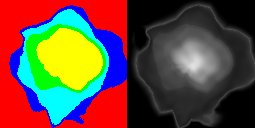
\includegraphics[width=0.6\linewidth]{terrainGAN.png}
	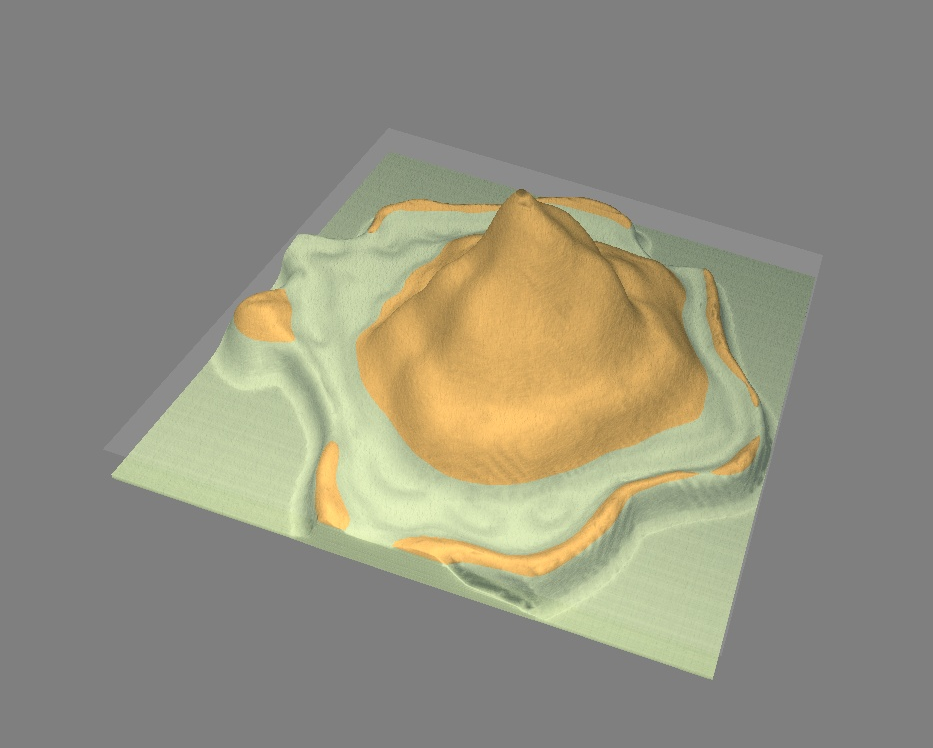
\includegraphics[width=0.3\linewidth]{terrainGAN_result.png}
	\caption{Caption.}
	\label{fig:teaser_cGAN}
}

\abstract 
In this chapter, we propose a procedural method for generating single circular volcanic islands using user sketching from two perspectives: a top view, which defines the island's shape (horizontal dimensions), and a profile view, which outlines its elevation and terrain (vertical dimensions). These perspectives, commonly used in geological and remote sensing domains, are complemented by a user-defined wind field, applied as a distortion field to deform the island's shape, mimicking the effects of wind and waves. Based on these inputs, our method generates a height field of the island. This algorithm is capable of creating many different island models, and we have generated thousands of exemplars to compose the dataset used for training a conditional Generative Adversarial Network (cGAN). By applying data augmentation, the cGAN allows for even greater variety in the generated islands, providing users with more control over the shape and structure of the final output.
\pagebreak 

\minitoc

\section{Introduction}
\label{sec:coral-island_introduction}

Coral reef islands are formed through a dynamic interplay of volcanic activity, coral growth, and long-term geological processes. These islands begin as volcanic landmasses, created when magma from the Earth's mantle erupts through the ocean floor and builds up layers of volcanic rock, eventually rising above sea level. In tropical waters, these volcanic islands create ideal conditions for coral reefs to develop. Corals, thriving in the shallow, sunlit waters around the island, initially form fringing reefs attached to the island's coastline.

As time passes, the volcanic island undergoes subsidence, a slow sinking process caused by the cooling and contraction of the Earth's crust beneath the island. In response to this subsidence, corals continue to grow upward, maintaining their position within the photic zone, where sunlight supports their survival. This upward growth leads to the formation of barrier reefs, which become separated from the island by a lagoon as the island sinks further.

Eventually, the volcanic island may submerge completely beneath the ocean's surface, leaving only the coral structure visible above water. This process results in the formation of atolls, which are ring-shaped reefs encircling a central lagoon. Over geological time, the physical structure of the island evolves from a prominent volcanic peak to a coral-dominated reef system, shaped by the combined forces of subsidence, coral growth, and erosion.

% 
Charles Darwin's subsidence theory, developed from his observations during the voyage of the HMS Beagle, remains one of the most widely accepted explanations for the formation of coral reef islands. Darwin proposed that coral reefs form around volcanic islands that slowly subside over time due to geological processes. As the volcanic island sinks, coral reefs grow upward, maintaining their position near the surface of the ocean. This theory explains the transition from fringing reefs attached to the island's coast, to barrier reefs separated by a lagoon, and finally to atolls, where the volcanic island has completely submerged, leaving only the coral structure visible above water.

While other theories, such as John Murray's growth on submerged mountains and Reginald Daly's sea level change theory, have also been proposed to explain coral reef formation, Darwin's subsidence theory remains the most widely supported due to its ability to account for the full evolution of coral islands, from volcanic landmasses to atolls. Its simplicity and focus on the relationship between subsidence and coral growth make it especially well-suited for computational modeling.

In our approach, we translate the core principles of Darwin's theory into a procedural generation model, simulating the gradual sinking of volcanic islands while coral reefs grow to keep pace with changing sea levels. This allows us to realistically model the transformation of islands from volcanic landmasses to coral-dominated atolls. By capturing this interplay, we can procedurally generate a wide variety of island structures that reflect real-world geological processes.

%

Simulating the formation of coral reef islands presents significant challenges due to the complex interplay of geological, environmental, and biological factors. One major difficulty lies in capturing the long-term subsidence of volcanic islands, which occurs over millions of years, while simultaneously modeling the upward growth of coral reefs that rely on environmental conditions such as water depth, temperature, and sunlight. This combination of slow geological processes and dynamic biological growth is difficult to replicate in a computational model.

Additionally, the biological aspects of coral growth are inherently tied to environmental factors. Coral reefs grow only within a specific range of water depth and sunlight, and their growth patterns are affected by the health of the reef ecosystem and the availability of resources. Accurately modeling these biological dependencies in a procedural system is challenging, as the factors governing coral reef development are difficult to generalize.

Existing terrain generation methods, such as Perlin noise-based algorithms or uplift-erosion models, are often ill-suited for these processes. While they can generate natural-looking landscapes, they do not account for the unique geological and biological interactions that govern coral island formation. Capturing these dynamics requires a balance between realism and procedural flexibility, allowing for both accurate simulation of natural processes and intuitive user control.

%

To address these challenges, we present a procedural generation tool that simulates the formation and evolution of coral reef islands by integrating both geological and biological processes. Our approach allows users to control the island's shape and structure through intuitive sketching interfaces, while the tool handles the complex dynamics of subsidence, coral growth, and environmental deformation.

The generation process begins with two user-defined inputs: a top view to outline the island's overall shape and a profile view to define its elevation and terrain contours. These inputs serve as the foundation for creating a height field of the island. Additionally, a wind deformation field allows the user to simulate the effects of wind and waves, reshaping the island's structure in a way that mimics natural erosion processes.

To enhance flexibility and allow for more complex, non-circular island structures, we incorporate a conditional Generative Adversarial Network (cGAN) into the generation process. The cGAN is trained on a dataset of islands generated by the initial algorithm, augmented to introduce a wider variety of shapes and features. This machine learning component allows for the automatic generation of diverse island models, removing some of the constraints of the initial procedural algorithm such as strictly radial symmetry while maintaining user control over key aspects of the design.

By combining user input with the adaptive power of the cGAN, our tool generates realistic coral islands that evolve from volcanic landmasses to coral-dominated atolls, capturing both geological and environmental processes.



\section{Overview}
Our system for generating coral reef islands combines user-driven sketching, procedural techniques, and deep learning to create realistic and varied island terrains. The process begins with the user sketching key features of the island, such as its overall shape and profile. This sketching process allows the user to define the layout of the island in an intuitive way, providing control over the placement of important elements like the island borders, beaches, lagoons, and coral reefs.

Once the user's sketch is complete, the system converts these high-level features into a labeled map, where each pixel is assigned to a specific region of the island. This map serves as the input to a conditional Generative Adversarial Network (cGAN), which is responsible for generating the fine details of the terrain. The cGAN has been trained on a dataset of island examples generated by the initial procedural algorithm, allowing it to produce realistic terrains that reflect the user's design while introducing natural variation and complexity.

By conditioning the cGAN on the user-defined map, the system maintains the overall structure and regions specified in the sketch, while generating realistic transitions between different areas (such as beaches, lagoons, and the island's interior). The use of deep learning, in combination with procedural techniques, allows the system to create coral islands that are both geologically plausible and tailored to the user's input.

This method provides a flexible yet powerful approach to island generation, enabling the creation of diverse island structures that reflect real-world geological processes, such as volcanic subsidence and coral reef growth.



\section{Related works}
Procedural generation of terrain has been a well-researched area in computer graphics and simulations, where the goal is to create large, realistic landscapes with minimal manual input. Various methods have been developed over the years to generate terrains automatically, from noise-based approaches to physically-based erosion simulations, sketch-driven methods, and more recently, deep learning techniques.

However, each of these techniques has its strengths and limitations, particularly when it comes to modeling coral reef islands. Coral islands present unique challenges due to the combination of long-term geological processes (such as subsidence and coral reef growth) and environmental interactions (like erosion caused by wind and waves). In this section, we review the key techniques that have been applied to terrain generation, highlight their limitations for coral island formation, and position our work as an approach that addresses these challenges.

\subsection{Noise functions}
% Noise functions
Noise-based procedural generation remains one of the most widely used techniques for creating natural-looking terrains. Introduced by Ken Perlin, the Perlin noise and Simplex noise are foundational algorithms that generates pseudo-random yet continuous variations across a grid, producing terrain features that resemble organic landscapes \cite{Perlin1985,Perlin2001}.

Beyond basic noise functions, more advanced techniques, such as Fractal Brownian Motion (FBM), are commonly used to add additional detail to terrains. FBM combines multiple layers, or "octaves," of noise at different frequencies, creating terrains with finer details and more realistic features. Noise functions are often paired with falloff maps to generate island-like terrains, where the height of the terrain gradually decreases toward the edges, mimicking the appearance of coastlines and providing a simple way to create basic island shapes.

Despite their widespread use, noise-based methods have significant limitations when applied to the simulation of coral reef islands. While these techniques excel at producing large, varied landscapes quickly, they lack the geological accuracy needed to model real-world processes like volcanic subsidence and coral growth. These approaches generate random patterns, but are disconnected from the actual physical processes that govern coral island formation.

Our approach goes beyond the randomness of noise-based generation by incorporating real-world geological and biological processes into terrain formation. Specifically, we model the gradual subsidence of volcanic islands and the upward growth of coral reefs, which are essential for representing the long-term evolution of coral reef islands. By integrating these processes into the generation algorithm, we create terrains that are not only more realistic but also allow for user control. This blend of user input and geological grounding provides a more accurate and flexible approach to modeling coral reef islands, addressing the limitations inherent in traditional noise-based techniques.

\subsection{Erosion simulation}
% Erosion simulation
While noise functions generate random, natural-looking terrain, they often fail to capture the physical processes that shape real landscapes over time. To address this limitation, erosion simulations model how natural forces such as water flow and gravity wear down terrain features, creating valleys, river networks, and other detailed landforms. These simulations are particularly effective at representing mountainous landscapes, where erosion gradually sculpts the terrain over long periods of time, typically on the scale of thousands to millions of years.

Erosion simulations often use models like the Stream Power Law to describe how water erodes higher elevations and deposits sediment in lower areas. The rate of erosion depends on factors such as slope steepness and water flow, with steeper slopes and greater water volumes leading to faster erosion. Over time, these processes create detailed and realistic terrain features like river valleys and erosion channels. Erosion models are iterative, simulating the gradual shaping of landscapes by continuously balancing forces like erosion and uplift, as seen in the work of \cite{Cordonnier2016,Cordonnier2017a}. Their model simulates how tectonic forces uplift terrain, which is then eroded away over thousands of years. Similarly, \cite{Schott2023} and \cite{Tzathas2024} refined the Stream Power Law to generate realistic slopes and ridges through these long-term geological processes.

Despite their effectiveness in modeling large-scale terrain evolution, erosion simulations are limited when it comes to representing environments that are shaped by dynamic biological processes. Coral reefs, for instance, grow and adapt to changing environmental conditions on a much shorter timescale than geological erosion. While erosion models simulate terrain changes over millennia, coral growth responds more dynamically to factors like water depth, light availability, and temperature on scales ranging from years to decades. These biological factors are difficult to incorporate into traditional erosion models, which are designed to simulate the slow, steady forces of water and gravity.

Our approach builds on the concept of terrain evolution by integrating the geological and biological dynamics that shape coral reef islands. Instead of focusing solely on erosion, which is primarily a surface-level process, we model the subsidence of volcanic islands over geological time and the simultaneous growth of coral reefs that adapt to the changing sea levels. Coral reefs must grow upward to remain within the photic zone, a process that unfolds on shorter timescales than those captured by standard erosion simulations. Furthermore, we introduce wind deformation to simulate the effects of environmental forces like wind and waves, which dynamically reshape the island's structure over time. This combination of long-term geological processes and short-term biological responses provides a more comprehensive simulation of coral reef island formation, capturing both the slow subsidence of volcanic landmasses and the rapid adaptability of coral ecosystems.

\subsection{Sketching}
% Sketching

In procedural terrain generation, sketch-based approaches allow users to directly interact with and shape landscapes through intuitive sketching interfaces. These methods enable users to define key terrain features such as mountains, valleys, and coastlines by drawing them in a two-dimensional canvas, which are then translated into 2.5D terrains. Sketching provides a high level of artistic control, making it especially popular in creative applications such as video games and simulations, where user-defined terrain features are prioritized.

Sketch-based systems offer great flexibility, allowing users to directly define specific elements of the landscape according to their needs or preferences. For instance, \citep{Gain2009} introduced a multi-perspective sketching system that allows users to generate detailed landscapes by sketching from different angles. This method provides more control over the terrain's shape than traditional noise-based generation methods. Similarly, \citep{Tasse2014} explored sketching from the player's viewpoint, allowing users to dynamically define height information from within the virtual environment, creating an interactive terrain design experience.

Sketching has also been extended to geological modeling. \citep{Patel2021} proposed a system where users can interactively model underground layers by sketching subsurface structures. This provides a powerful tool for geologists and designers who need to model complex, multi-layered terrains, offering more control over both the surface and the subsurface.

In our work, we leverage the flexibility of sketching to define the key features of coral reef islands, such as the island shape, lagoons, and coral reefs, in a vectorized format. This is particularly important for modeling underwater and island landscapes, where these features are not simply surface elements but part of an evolving geological structure. By using sketches, we retain the semantic information of where the island and coral regions are located, which allows us to later apply our simplified model of Darwin's subsidence theory.

Rather than focusing on detailed long-term or short-term evolution, our method adapts sketching to the unique requirements of island and underwater landscapes. Once the user defines the terrain layout through sketching, we apply a simplified subsidence model, where the volcanic island gradually sinks and coral reefs grow in response, remaining close to the water surface. This process provides a framework for simulating the evolution of the landscape in a geologically plausible manner.

The key advantage of sketching in our system is that it combines the artistic control provided by traditional sketching methods with the ability to handle the geological processes specific to coral reef islands. By preserving the vectorized information from the sketch, we can accurately place and evolve features like lagoons and coral reefs, ensuring that the resulting terrain reflects both the user's design intent and the geological dynamics at play.

\subsection{Deep learning}
% cGAN

In recent years, deep learning has become a transformative tool in computer graphics, image processing, and procedural content generation. Deep learning refers to a class of machine learning techniques that use artificial neural networks with multiple layers to model complex patterns in data. By training these networks on large datasets, deep learning models can learn to generate new, realistic data by identifying the underlying relationships between inputs and outputs.

In terrain generation, deep learning is particularly well-suited to tasks that require the creation of complex, natural-looking landscapes. Traditional procedural generation techniques like noise functions and erosion simulations can be powerful, but they often struggle to produce the complexity and realism of natural terrains due to their reliance on predefined rules and algorithms. In contrast, deep learning models, especially Generative Adversarial Networks (GANs), can learn from data, enabling them to generate realistic terrains that mimic the diversity and complexity found in nature.

GANs are a particularly effective deep learning architecture for terrain generation. A GAN consists of two neural networks: a generator, which creates new data samples, and a discriminator, which evaluates whether the generated samples are real or fake compared to a set of training data. Through this adversarial process, the generator gradually improves its ability to produce realistic examples, while the discriminator becomes better at distinguishing real from fake data. This feedback loop allows GANs to generate highly realistic and detailed terrain features by learning from large datasets of existing terrains.

In terrain generation, GANs have been applied to generate diverse landscapes by learning the patterns and features found in real-world terrains. For example, \citep{Guerin2017} demonstrated how GANs can be used to transform 2D sketches into 3D terrains by training the network on a dataset of terrain features, allowing the system to generate new landscapes based on simple user input. GANs are particularly well-suited for this task because they can capture the subtle details of terrain that would be difficult to model explicitly, such as the natural flow of elevation or the transitions between different terrain types.

A variant of GANs, known as Conditional Generative Adversarial Networks (cGANs), takes the power of GANs one step further by allowing the generated data to be conditioned on additional inputs. In a cGAN, both the generator and the discriminator receive additional information such as a class label, a sketch, or an image, that guides the generation process. This makes cGANs particularly useful for terrain generation tasks where users want to control specific aspects of the output while still relying on the model to generate realistic details.

In the case of terrain generation, a cGAN allows the user to specify high-level constraints (such as the outline of an island or the regions where different terrain types should be) while the generator fills in the finer details based on what it has learned from the training data. This makes cGANs particularly effective in applications where a mix of user input and data-driven generation is required, as the user can control the broad layout of the terrain while the model ensures that the resulting terrain looks natural and plausible.

In our approach, we use a cGAN to generate coral reef islands, providing a balance between user control and realistic terrain generation. After the initial algorithm outlines the regions of the island such as the island itself, beaches, and lagoons, these regions are transformed into a single image, where each pixel represents a different region ID. This image is used as the input for the cGAN, which conditions the generation process on this initial layout.

The cGAN is trained on a dataset of island examples, which are created by the initial procedural generation algorithm and further augmented to introduce a wide variety of shapes and features. This training allows the cGAN to generate coral reef islands that follow the high-level layout provided by the user while introducing natural variations and details that reflect real-world island characteristics. By conditioning the cGAN on the user-defined region map, we ensure that the generated islands maintain structural coherence while still exhibiting realistic features like smooth transitions between regions, varied terrain, and non-circular shapes.

One of the key advantages of using a cGAN in our system is its ability to overcome procedural constraints. Traditional procedural generation methods often impose limitations like radial symmetry or require islands to follow overly simplified geometries. With the cGAN, these constraints are lifted. The model can generate irregular, non-circular islands that adhere to the user's input but introduce a level of complexity and realism that would be difficult to achieve with purely procedural methods.

Additionally, the cGAN ensures that the generated island terrain aligns with the geological processes modeled in the system, such as subsidence and coral reef growth. By training the cGAN on thousands of examples that reflect these processes, we ensure that the final generated island models are both flexible and geologically plausible. The combination of user-driven design and data-driven generation through the cGAN allows for the creation of coral reef islands that are not only tailored to the user's input but also realistic in their form and structure.



\section{Example generation}
\label{sec:coral-island_example-generation}

Generating synthetic coral reef island terrains involves a combination of user input, procedural techniques, and simplified geological simulations. The process begins with the creation of a base terrain using user-defined sketches, followed by a simulation of coral reef growth and subsidence. These two steps, although interconnected, can also be used independently, providing flexibility in how the system is applied. In this section, we describe the example generation process in detail.

\subsection{Assumptions}
In generating synthetic coral reef islands, we adopt a set of simplifying assumptions that are grounded in geological and biological observations. These assumptions streamline the process while producing plausible terrains. Below, we outline the key characteristics of our model:

% \begin{itemize}
    \textit{Radial symmetry:} Volcanic islands often begin as circular landmasses due to the radial uplift of magma from beneath the Earth's mantle. Erosion processes further smooth out sharp edges over time, reinforcing this initial symmetry. In our approach, we assume islands start with an approximately circular shape, providing a straightforward basis for terrain generation.
% This assumption reflects real-world volcanic islands, such as those in the Pacific, where erosion gradually shapes the initial circular form. Starting with a radial structure simplifies the generation and serves as a solid foundation for further deformation.

    \textit{Coral growth at constant depth:} Coral reefs require sunlight to thrive, which limits their growth to depths where light penetrates the water. In our model, coral growth is constrained to this depth range, with corals maintaining their proximity to the water surface as the volcanic island subsides.
% Coral growth follows biological principles, growing upward in shallow waters. This assumption simplifies the process of modeling coral features and reflects the observed behavior of real coral reefs.

    \textit{Radial arrangement of features:} The key island features like the island body, beaches, lagoons, and coral reefs, are arranged in concentric regions around the island center. This radial arrangement aligns with natural geological progression from the island to the surrounding reef.
% This simplifies the generation process by organizing features in a predictable order, similar to coral atolls where lagoons and reefs form protective rings around the island.

    \textit{Wind and wave deformation:} Over time, wind and wave forces shape islands by introducing concave regions, carving out lagoons, and deforming coastlines. To simulate these effects, we apply a wind deformation field that allows users to introduce natural variations that break the radial symmetry, resulting in more realistic island shapes.
% Wind and wave erosion play a significant role in shaping real coral islands, and simulating this erosion adds natural-looking variation. The wind field gives the user control over how much deformation is applied, creating non-uniform, dynamic island coastlines.

    \textit{Independence of islands:} In this model, each island is treated as an independent entity, meaning its terrain does not influence neighboring islands. This allows multiple islands to be generated and placed freely without concern for terrain overlap or interaction. 
% This assumption reflects the typical formation of islands in archipelagos, where individual islands are geographically separate. It simplifies the generation of multi-island scenes by avoiding unnecessary inter-island interactions.

    \textit{Uniform profile shape:} We assume that the vertical profile of the island remains relatively uniform, meaning that the terrain's cross-section from the center outward is similar in every direction. This allows for consistent scaling of the profile in all directions, ensuring that the island's shape remains coherent and plausible.
% Although real-world islands can have local variations in their profile, this uniformity makes the generation process more manageable and produces consistent terrain features.

    \textit{Subsidence and coral growth:} As the volcanic island subsides, coral reefs grow to keep pace with the sinking landmass, maintaining their height near the water surface. In our model, the island subsides as a whole, while coral features are preserved by growing vertically. This separation allows the coral regions to remain unaffected by the subsidence of the island itself.
% This assumption is based on Darwin's subsidence theory, which explains the formation of coral atolls. Modeling coral growth independently of the island's subsidence ensures the coral regions stay at the water surface as the island sinks.
% \end{itemize}

These assumptions, while simplified, provide an effective foundation for generating coral reef islands. They balance computational efficiency with geological plausibility, ensuring that the generated terrains are both flexible and realistic. Furthermore, the system allows users to break the radial symmetry and introduce more natural variations through wind deformation, adding another layer of flexibility to the model.


\subsection{User Input}

The generation of coral reef islands in this system begins with two intuitive sketch-based inputs from the user: a top-view sketch and a profile-view sketch, which define the islands horizontal layout and vertical elevation profile. In addition to these sketches, the user can further refine the terrain by applying wind deformation strokes, which simulate the effects of wind and waves on the islands shape. This combination of sketches and wind inputs gives users precise control over both the islands structure and its natural variations, such as irregular coastlines or concave features.

\subsubsection{Top-view Sketch}

The top-view sketch defines the islands outline as seen from above. Using a simple drawing interface, the user can delineate the boundaries between key regions of the island, including the island itself, the beaches, the lagoon, and the surrounding abyss. The system assumes that these regions are arranged concentrically around the center of the island, with each boundary defined by a radial distance from the center.

Each region's boundary is represented in polar coordinates, with $\radius_\p$ indicating the radial distance from the islands center and $\theta_\p$ representing the angular position. This polar representation allows the system to map the users sketch onto a circular framework, ensuring smooth transitions between regions and maintaining a coherent layout for the island.

In this sketch, the user defines the overall horizontal layout of the island, including the size and shape of each feature. Variations in the outline can be introduced by allowing the radial distances to vary with angle, ensuring that the island is not strictly symmetrical and introducing more natural, irregular shapes.

\subsubsection{Profile-view sketch}

The profile-view sketch defines the vertical elevation profile of the island along any radial direction, offering control over the islands height. In this view, the user specifies the elevation of different regions of the island, such as the island peak, beach, lagoon, and abyss, by marking a set of milestones along the profile.

These milestones correspond to key terrain transitions: the highest point of the island (center), the island border, the beach, the lagoon, and the deep-sea abyss. The system uses these milestones to interpolate a continuous 1D height function $\heightProfile(x)$, where $x \in [0,1]$ represents the normalized radial distance from the islands center, and $h = \heightProfile(x)$ gives the height at each point. This continuous profile ensures smooth elevation transitions across the island.

By combining the top-view and profile-view sketches, the system can generate a full 3D terrain model that accurately reflects the users design.

\subsubsection{Wind velocity field}
In addition to the sketches, the user can influence the shape of the island by defining a wind velocity field. This field simulates the effects of wind and wave erosion on the island's surface, introducing natural deformations such as coastline indentations, concave features, or variable lagoon shapes.

The wind field is represented as a series of wind strokes drawn by the user on a 2D canvas. Each stroke represents a parametric curve, where the direction and strength of the wind are encoded as a vector field. The user controls the wind's direction by drawing these curves, and the system interprets the strokes to create a velocity field that defines how the terrain should be deformed.

As the user draws a wind stroke, the system generates a set of control points along the curve, with the option to adjust the stroke's width. The width of each stroke determines the area of influence around the curve, where wider strokes result in broader deformations of the terrain.
The deformation strength decreases with distance from the wind curve using a Gaussian falloff function using the stroke width as standard deviation, ensuring that the terrain transitions smoothly from deformed regions to non-deformed areas.
Once the wind strokes are applied, the system processes the wind velocity field by displacing the terrain points accordingly. The height field, originally generated from the user's sketches, is modified by the wind field to create non-radial features, breaking the initial radial symmetry and producing a more organic island shape.

\subsubsection{User interaction}

As users draw the top-view and profile-view sketches, the system provides real-time feedback on the resulting terrain. The top-view sketch influences the horizontal layout of the island, while the profile-view sketch defines its vertical structure. These sketches can be adjusted independently, allowing the user to fine-tune both the outline and elevation of the island.

After sketching the basic shape, users can apply wind deformation strokes to modify the island's features further. These strokes represent wind and wave influences, distorting the island's shape to introduce more natural, non-radial features such as indentations along the coastline, variable lagoon shapes, or concave formations. The system automatically applies these deformations, providing real-time feedback as the user interacts with the terrain.

This interactive process, combining sketches and wind deformation, allows users to quickly iterate on their designs, refining the terrain to meet specific aesthetic or functional goals.




\subsection{Generation process}
The generation of coral reef island terrains involves a structured process that takes the user's sketches and produces a complete 3D terrain model. This process begins with the creation of the initial height field based on the user's input, followed by the application of wind deformation to introduce natural variations, and concludes with the integration of coral reef features through subsidence and coral growth modeling.

\subsubsection{Initial height field generation}
The generation of the coral reef island terrain begins by transforming the user-defined top-view and profile-view sketches into a coherent 3D height field. This process combines the radial layout of the top-view sketch with the elevation information provided by the profile-view sketch, creating a terrain that accurately represents the desired features, such as the island, beaches, lagoons, and abyss.

For any point $\p$ on the terrain, the system first computes the polar coordinates $(\radius_\p, \theta_p)$, where $\radius_\p$ is the radial distance from the island's center, and $\theta_p$ is the angular component. The radial distance $\radius_\p$ is used to determine which region the point belongs to (island border, beach, lagoon, or abyss). The user-defined milestones in the profile sketch specify the radial boundaries between these regions.

Each point's height is determined by the profile function $\heightProfile(x)$, where $x$ represents the normalized radial distance from the island's center. The function $\heightProfile(x)$ is continuous and defines the height of the terrain at any point along the profile, from the island's center (at $x = 0$) to the outer boundary of the abyss (at $x = 1$).

The system first identifies which region the point $\p$ falls into by comparing $\radius_\p$ with the radial boundaries defined by the milestones. These milestones divide the terrain into sections, such as:
\begin{itemize}
    \item Island: $\radius_\p \leq \radius_{\text{island}}$,
    \item Beach: $\radius_{\text{island}} < \radius_\p \leq \radius_{\text{beach}}$,
    \item Lagoon: $\radius_{\text{beach}} < \radius_\p \leq \radius_{\text{lagoon}}$,
    \item Abyss: $\radius_{\text{lagoon}} < \radius_\p \leq \radius_{\text{max}}$
\end{itemize}

For any point between two milestones (e.g., between the island border and the beach), the system computes the normalized distance $x_\p$ using linear interpolation between the radial distances of the two milestones. For example, if $\radius_\p$ is between the beach boundary $\radius_{\text{beach}}$ and the lagoon boundary $\radius_{\text{lagoon}}$, the value of $x_\p$ is computed as:

\begin{align}
    x_\p = \frac{\radius_\p - \radius_{\text{beach}}}{\radius_{\text{lagoon}} - \radius_{\text{beach}}}
\end{align}

This normalized distance $x_\p$ represents the position of point $\p$ relative to the region's boundaries.

Once the correct value of $x_\p$ is determined, the height of the point $h(\p)$ is computed directly using the profile function $\heightProfile(x)$, which smoothly defines the height for any given value of $x$. The height function $\heightProfile(x)$ is continuous across all regions, ensuring that transitions between the island, beach, lagoon, and abyss are smooth.

For any point $\p$, the height is computed as:
\begin{align}
    h(\p) = \heightProfile(x_\p)
\end{align}

This approach ensures that the height field accurately follows the elevation profile specified by the user while maintaining smooth transitions between different regions of the island.

By using the profile function $\heightProfile(x)$ to directly compute the height for any point on the terrain, the system guarantees smooth transitions between regions (e.g., from the island to the beach or from the lagoon to the abyss). This method eliminates the need for separate interpolation between regions, as the function $\heightProfile(x)$ is defined continuously across all regions of the island.

The result is a height field that captures both the radial structure of the island (from the top-view sketch) and the vertical elevation profile (from the profile-view sketch), producing a realistic representation of coral reef islands with smooth transitions between the key terrain features.



\subsection{Wind deformation}

After generating the initial height field based on the top-view and profile-view sketches, the next step in the process introduces wind deformation. This step simulates the long-term effects of wind and wave erosion, breaking the radial symmetry of the terrain and adding natural variations such as concave coastlines and irregular island shapes.

% \subsubsection{User-defined wind field}

The wind deformation can be controlled through a user-defined vector field, which represents the direction and strength of wind flows across the terrain. Users interact with the system by drawing strokes on a 2D canvas, which are then interpreted as parametric curves $\curve$ representing wind patterns. Each stroke defines a wind flow in the curve's direction $\curve'$ and an effect width $\std$, and these wind flows are used to displace the terrain, simulating the gradual reshaping of the island due to wind and wave erosion.

The strokes are represented as Catmull-Rom splines, a type of parametric curve that allows for smooth, continuous wind paths. For any point $\p$ on the terrain, the deformation vector $\warp(\p)$ is calculated based on the proximity of $\p$ to the nearest wind strokes. The strength of the displacement is controlled by a Gaussian scaling function, which ensures that points closer to the wind strokes experience stronger displacement, while points farther away are less affected.

The displacement $\warp(\p)$ is computed as a sum of the influences from all nearby wind strokes. For each stroke, the deformation vector is scaled by a Gaussian function that decreases with the distance from the closest point $\q$ on the parametric curve $\curve$, as follows:

\begin{align}
    \warp(\p) = \sum_{\curve \in \text{curves}} \curve'(\q) \cdot e^{-\frac{\norm{\p - \q}^2}{2 \std^2}}
\end{align}


% \subsubsection{Deformation process}
Once the deformation vector $\warp(\p)$ is computed, the terrain height at point $\p$ is adjusted by displacing $\p$ to a new point $\warp(\p)$.
We can then compute the final height $h(\warp \circ \p) = \heightProfile(t_{\p})$, or, as the implicit modeling community would write it, 
\begin{align}
    \Tilde{h}(\p) = \warp^{-1} \circ h
\end{align}

This process introduces variations in the terrain, distorting the coastline, creating concave regions, and breaking the original radial symmetry defined by the top-view and profile-view sketches.

\subsubsection{Resistance to deformation}

To ensure that certain regions of the terrain, such as deep-water areas, remain relatively unaffected by the wind, a resistance function $\rho(x)$ is applied. The resistance function modulates the effect of the wind deformation based on the radial distance $\radius_\p$ from the island's center, which is normalized to a value $x \in [0, 1]$.

The resistance function $\rho(x)$ is defined similarly to the profile function, and it controls the magnitude of the displacement at each point. For example, regions near the coastline (such as the beach and lagoon) might have lower resistance, allowing for more significant deformation, while regions farther away (such as the abyss) have higher resistance, limiting the wind's impact.

The deformation vector is scaled by the resistance function at each point $\p$, such that the final deformation vector becomes:

\begin{align}
    \Tilde{\warp}(\p) = \rho(x_\p) \cdot \warp(\p)
\end{align}

Where $\rho(x_\p)$ is the resistance value corresponding to the point's normalized distance $x_\p$. This ensures that the wind deformation has the greatest impact on areas like the coastline and beach, where erosion naturally plays a larger role, while deeper regions like the abyss remain stable and relatively unchanged.

\subsubsection{Deformation and height field update}

The wind deformation process results in a modified height field where the terrain has been warped according to the user-defined wind strokes. This deformation introduces non-radial features, such as concave coastlines or irregularities along the beach and lagoon, making the island appear more natural and varied.

Both the height field and the labeled map (which tracks the terrain regions like island, beach, and lagoon) are updated to reflect the wind deformation. This ensures that the semantic information of the terrain remains consistent even after the terrain has been warped. The labeled map is deformed in the same way as the height field, preserving the logical structure of the island for further post-processing, such as texturing.

For instance, consider a simple circular island generated from the initial height field. By applying wind strokes along one side of the island, the deformation process can create concave regions along the coastline, making the shape more irregular and mimicking the effects of real-world wind and wave erosion. The resistance function ensures that while the beach and lagoon areas are deformed, the abyss remains largely unaffected as they are far from the wind and wave effective areas, preserving the island's overall structure.




\subsection{Coral reef modeling}

Once the terrain has been generated and deformed by the wind, the system simulates the subsidence of the volcanic island and the growth of coral reefs. These processes reflect the long-term geological evolution of coral reef islands, where the volcanic island gradually sinks (subsides) while coral reefs grow upward to keep pace with the sinking landmass.

\subsubsection{Subsidence}

The subsidence of the island is modeled by scaling the initial height field downward, simulating the effect of the volcanic island slowly sinking into the ocean. The user provides a subsidence rate $\lambda$, which represents the proportion by which the island has sunk over time. The subsidence is applied uniformly to the terrain, meaning all points on the island sink by the same factor.

The subsided height field $h_{\text{subsided}}(\p)$ is computed by scaling the original height field $h_0(\p)$ with the subsidence factor $\lambda$:

\begin{align}
h_{\text{subsided}}(\p) = (1 - \lambda) \cdot h_0(\p)
\end{align}

Where:
- $\lambda \in [0, 1]$ is the subsidence rate (e.g., $\lambda = 0.2$ means the island has subsided by 20% of its original height),
- $h_0(\p)$ is the height at point $\p$ from the initial height field.

This scaling reduces the overall height of the island, simulating how volcanic islands sink over time due to tectonic activity and erosion. The subsidence factor $\lambda$ is applied uniformly across the terrain, meaning that all points on the island experience the same degree of subsidence, regardless of their original height or location.

\subsubsection{Coral reef growth}

As the volcanic island subsides, coral reefs grow upward to remain close to the water surface, following the “keep-up” strategy observed in real-world coral formations. Coral growth is restricted to regions where the depth is within the optimal range for coral development, typically from the water surface to around 30 meters below.

The coral reef features (reef crest, back reef, and fore reef) are modeled separately from the subsidence process. The system generates a coral feature height field $h_{\text{coral}}(\p)$, which remains unaffected by the island's subsidence. This height field ensures that coral regions remain near the water surface, even as the island sinks.

Coral reef growth is entirely independent of the subsided terrain. Even as the volcanic island sinks, coral growth is driven only by the proximity of terrain to the water surface, ensuring that coral features always remain near the surface, irrespective of how much the island subsides.

The coral reef height field is generated using predefined depth values for the various coral regions:
- The reef crest is modeled near the water surface, typically just below sea level,
- The back reef and lagoon are slightly deeper but remain within the range where corals can grow,
- The fore reef slopes downward into the deep ocean, transitioning into the abyss.

The system uses these predefined regions to assign heights to coral reef points based on their proximity to the reef crest. For example, the height of a point in the fore reef is interpolated between the reef crest height and the deeper abyss regions.

\subsubsection{Blending the height fields}

The final step is to blend the subsided height field $h_{\text{subsided}}(\p)$ with the coral feature height field $h_{\text{coral}}(\p)$ to produce the final terrain. The goal is to ensure that coral features remain near the water surface while allowing the rest of the island to subside.

To achieve this, the system uses a smooth max function, which smoothly blends the two height fields. The smooth max function ensures that the coral regions dominate where coral growth is present, while the subsided island terrain dominates in other regions. This blending method ensures that the transition between the coral and subsided regions is smooth and visually consistent.

The smooth max function adapted from Ingo Quilez's smooth min function is defined as:

\begin{align}
    \smoothmax(a, b, k) = a + \frac{(b - a)}{1 + \exp\left(-k \cdot (b - a)\right)}
\end{align}

Here, $a = \heightSubsid(\p)$ is the height from the subsided island, $b = \heightCoral(\p)$ is the height from the coral reef feature, and $k$ controls the smoothness of the transition.

This smooth max function guarantees visual continuity by preventing abrupt height differences between the coral regions and the subsided terrain, creating a smooth, gradual transition that mimics the natural blending of coral reefs with deeper areas. The coral feature height field takes precedence where coral can grow, typically in shallow regions up to around 30 meters below the water surface. In deeper regions, such as the abyss, the subsided height field naturally dominates, ensuring that the final terrain accurately reflects both subsidence and coral growth processes.

\subsubsection{Output}

The resulting terrain represents a realistic coral reef island, where the volcanic island has subsided, and coral reefs have grown upward to keep pace with the water level. The smooth blending between the subsided terrain and the coral features ensures a natural transition between regions like the island, lagoon, and coral reefs.

One of the key strengths of this method is its flexibility: 
- The subsidence and coral reef growth processes are modeled independently, allowing for a wide range of configurations. Users can generate plausible island terrains with or without coral features, or apply the coral reef growth simulation to existing height fields from other sources.
- Additionally, the coral reef growth simulation can be fine-tuned by adjusting the predefined depth values for different coral regions, allowing for further customization of the terrain's appearance.





\section{Conditional Generative Adversarial Networks}

In this section, we introduce the use of a Conditional Generative Adversarial Network (cGAN), specifically the pix2pix model, to enhance the island generation process by increasing the variety and flexibility of terrains. While the initial procedural algorithm can create numerous island examples, cGAN provides additional flexibility in generating more complex terrain without the rigid constraints of the first algorithm.

\subsection{Introduction to cGAN}

A Generative Adversarial Network (GAN) consists of two competing neural networks: a generator that attempts to produce realistic data, and a discriminator that tries to distinguish between real and generated data. In the conditional GAN (cGAN) variant, both the generator and discriminator are conditioned on some input, meaning the generated output is influenced by additional information, such as a labeled map or image.

For island generation, we use the pix2pix model, a specific cGAN designed for image-to-image translation. In this case, the input to the generator is a labeled map which is a 2D image where each pixel is assigned an ID representing a different region of the island (e.g., island body, beach, lagoon, coral reef). The output is an image where each pixel corresponds to the elevation of the terrain at that point, ie. a height field.

\subsection{cGAN for island generation}

The cGAN model was chosen for this task because it allows us to overcome some of the constraints of the initial procedural algorithm. While the first algorithm generates island terrains based on radial symmetry and a limited set of input parameters, cGAN can generate more complex and varied terrains by learning from a large dataset of examples. Specifically, the use of cGAN addresses the following challenges:

1. Increased Variety: The cGAN model can generate a wide range of island shapes and terrains by learning from the dataset. This allows for the creation of terrains that go beyond the predefined structures of the initial algorithm, introducing more natural variation in island features.

2. Overcoming Constraints: In the initial algorithm, islands are always centered in the image and adhere to a radial symmetry. Using cGAN, we apply data augmentation (translation, scaling, and combining multiple islands in one sample) to remove these constraints, allowing islands to take more irregular shapes and positions.

3. Flexibility: Once trained, the cGAN model acts as a black box that generates island terrains based on the labeled input. While this limits user control during the generation process, the model can produce a variety of terrains that still respect the underlying structure of the labeled map. This enables a flexible, rapid generation process without requiring the user to fine-tune parameters manually.

\subsection{Training}

The cGAN model is trained using a dataset of island terrains generated by the initial algorithm. To create this dataset, the algorithm randomly generates top-view shapes for the island's features, adds noise (such as fractional Brownian motion, or fBm), and introduces random wind velocity fields. The profile function remains consistent in determining the relative positions of the island, beach, and lagoon, but the top-view shapes vary through noise and deformation.

\subsubsection{Data augmentation}

To enhance the variety of the dataset and improve the model's ability to generalize, we apply several data augmentation techniques:
- Translation: Since the original algorithm always centers the island, we translate the islands within the image to remove this constraint. This ensures that the cGAN can generate islands in any position within the frame.
- Directional Scaling: By scaling the terrain in one direction, we create elongated islands that resemble corridors or archipelagos, adding another layer of diversity to the dataset.
- Multiple Islands per Sample: In some cases, we combine multiple islands into a single sample, ensuring they do not overlap. The regions not covered by any island are assigned the abyss ID. Although this approach ensures non-overlapping regions, future work could explore using blending techniques to position islands more closely without the risk of overlap.

All augmentation techniques are applied both to the height field and the labeled map simultaneously to ensure consistency between the input (labeled map) and the output (height field).

\subsection{Model output}

Once trained, the cGAN model generates a height field from a given labeled map. The output is a complete 2D height map representing the terrain's elevation at each point. Although the cGAN works as a black box, the labeled map remains available after inference and retains valuable information for the user.

The labeled map can be used for post-processing tasks, such as:
\begin{itemize}
    \item Texturing: Different regions of the terrain (e.g., beach, lagoon, coral reef) can be textured based on their region ID from the labeled map, allowing for detailed terrain decoration.
    \item Material Information: The labeled map can provide cues about the underlying ground material in each region, which can be useful for additional simulations, such as erosion or weathering.
\end{itemize}

However, it's important to note that the current implementation of the cGAN does not allow for user control during the generation process itself. The model takes the labeled map as input and outputs a height field without any additional parameters that the user can adjust in real-time. While this limits user interaction, the resulting terrains are still varied and flexible thanks to the data diversity learned during training.

\subsection{Limitations}

While the cGAN model provides increased flexibility and variety in island generation, it does come with certain limitations:

\begin{itemize}
    \item Biases from the synthetic dataset: Since the cGAN model is trained entirely on a procedurally generated dataset, it inherits the biases present in the initial algorithm. For example, while the model can break free from the radial symmetry constraint and center positioning, it still relies on the synthetic data's structure and patterns. This can limit the true diversity of the generated terrains, as the cGAN cannot generate terrains that deviate too far from the examples in the training set.
    \item Lack of user control: Another limitation of using cGAN in this context is the lack of real-time user control during terrain generation. While traditional procedural generation methods allow users to tweak parameters (e.g., island size, beach width) during the generation process, the cGAN model operates as a black box, providing no mechanism for direct user interaction beyond the initial labeled map. This reduces the level of customization available to the user.
    \item Data-driven dependence: The quality of the generated terrain depends entirely on the quality and variety of the training dataset. Since the dataset is synthetically generated, any limitations or biases in the initial dataset directly affect the cGAN's output. This dependence on data quality makes it crucial to design a well-augmented and varied dataset to ensure diverse and realistic outputs.
\end{itemize}



\section{Conclusion}

This work has presented a novel approach to generating coral reef island terrains by combining traditional procedural methods with deep learning techniques. We first developed a procedural generation algorithm capable of creating a wide variety of island terrains through a combination of top-view and profile-view sketches, wind deformation, and subsidence and coral reef growth simulation. By applying these methods, we were able to produce realistic terrains based on geological processes, capturing key features of coral reef islands such as beaches, lagoons, and coral reefs.

To further enhance flexibility and realism in the generation process, we incorporated a Conditional Generative Adversarial Network (cGAN), using the pix2pix model to generate height maps from labeled maps of island features. The cGAN model allowed us to overcome some of the constraints inherent in the procedural algorithm, such as radial symmetry and fixed island positioning. With data augmentation techniques, we were able to train the cGAN on a synthetic dataset, generating varied and realistic island terrains.

\subsection{Advantages of the approach}

One of the main strengths of this approach is its ability to produce a wide variety of island terrains, even in the absence of real-world data. The procedural generation methods allow for high flexibility in designing both the shape and features of the island, while the use of cGAN enables further refinement and the generation of terrains that are not bound by the original constraints of the procedural model. By combining these two methods, we leverage the advantages of both: the structured control of procedural techniques and the pattern-learning capabilities of deep learning.

A key advantage of this approach is the retention of semantic information about the terrain throughout the generation process. The labeled map, which serves as the input to the cGAN, can also be used after terrain generation to provide a detailed representation of the different regions of the island (such as the beach, lagoon, coral reef, and island body). This labeled map can guide post-processing operations, such as applying different textures based on terrain features or adding other environmental elements like vegetation. The preservation of semantic information provides a useful connection to the next stage of terrain manipulation, making the process more versatile and adaptable to different use cases.

Furthermore, the use of an out-of-the-box cGAN model highlights the feasibility of employing existing neural network architectures with minimal modifications in the field of procedural generation. This is particularly important in domains where real-world data is scarce, such as coral reef islands, allowing synthetic data to be effectively used for training purposes.

\subsection{Limitations}

While this approach brings significant advantages, there are also some limitations to consider. The reliance on a synthetic dataset means that the cGAN inherits the biases and limitations of the original procedural algorithm. This could limit the true diversity of the terrains that the model can generate, as the output is confined by the patterns present in the training data. Additionally, the cGAN model functions as a black box, offering limited user control over the generation process once the model has been trained. This contrasts with traditional procedural methods, which typically allow for real-time tweaking of parameters.

\subsection{Future works}

There are several directions for future research and improvements. One promising avenue is to incorporate the wind velocity field more directly into the cGAN training process, potentially as an additional input condition. This would allow the model to better capture wind-driven terrain features such as cliffs or other deformations influenced by wind patterns.

Another area for exploration is improving user interaction during the terrain generation process. While the current model allows for rapid terrain generation, adding more options for users to interact with the cGAN, such as tweaking parameters like wind strength or island size, could enhance the flexibility of the system.

Finally, further improvements could be made to the synthetic dataset. Incorporating more complex geological processes, such as wave erosion or tidal influences, could lead to even more realistic terrains. Additionally, refining the way islands are blended in multi-island samples, or adding more diverse input conditions (e.g., different geological settings), could help the model generalize better and produce more varied and dynamic landscapes.


One possible future improvement could involve incorporating the wind velocity field into the cGAN training process. While the labeled map is the only input used in the current implementation, the wind field could be added as an additional condition. This would be especially useful if the initial algorithm were augmented to include wind-driven features, such as cliffs or specific terrain deformations influenced by wind patterns. Adding the wind field as an input could help the cGAN generate more realistic terrains that better reflect the influence of wind on the landscape.

Additionally, further development could explore improving how multiple islands are combined in a single sample. For example, using blending techniques to handle overlapping regions could allow islands to be positioned closer together, enabling the generation of more complex archipelagos without sacrificing the integrity of the height field.


\graphicspath{ {./Chapter 1/} }

\chapter{Semantic terrain representation}
\label{chap:semantic-representation}
\teaser{
    \includegraphics[width=0.9\linewidth]{Figures/Render/figureTeaser.png}
	%  % \centering
    \caption{Our method can produce different scenes including coral reef islands and canyons at multiple scales using \glosses{EnvObj} to represent terrain features.}
	\label{fig:semantic-representation_teaser}
}
\abstract
\label{chap:semantic-representation_abstract}
% - Terrain generation usually focus on geometry processing \\
% - Some works include soil materials in their process \\
% - But no semantic information is preserved \\
% - Many fields use topologic maps to describe the environment \\
% ** see Travel books \\
% - Our method to abstract the geometry and focus on the symbolic \\
% - ... 
This chapter introduces a novel method for procedural terrain generation, which leverages a sparse representation of environmental features to produce landscapes that are lightweight, plausible and adaptable to user desires. The method differs from traditional terrain generation approaches by emphasizing multi-scale user interaction and incorporating expert knowledge to model the evolution of terrain features over time. By representing terrain features as discrete entities, or "\glosses{EnvObj}", the method enables dynamic interaction between these entities and their surrounding environment, represented through continuous scalar and vector fields. The generation process is iterative and allows for user-guided modifications at any iteration, including the introduction of environmental events that can influence the terrain's evolution. The proposed approach is particularly flexible, capable of generating both terrestrial and underwater landscapes with a focus on large-scale plausibility and detailed, localized feature representation. 
\pagebreak 

\minitoc

% topography
% Representing an environment as a topographic map
% A method that uses new objects, EnvObjs, to represent the landmarks of a terrain
% Our method represents the different landmarks of a terrain using a geometric (as "without 3D repr") representation. To avoid cycles in the interactions between objects, we use the environment as a proxy. EnvObjs are independant, like cellular automata. Each object affects locally the environment by modifying EnvVals. This modifications are applied by the EnvObjs spreading EnvMat around them. They also absorb EnvMat from the other EnvObjs. We can consider that the diffusion is bounded thanks to a decay rate, meaning the system becomes stable after some time. Because it is stable, it is plausible. We break the stability by adding new EnvObjs following \glosses{GenRule}. New EnvObjs are placed in the environment where they may be the most probable, following a fitness function using the EnvVals. Then the shape of the skeleton is defined following a skeleton \gloss{FitnessFunc}. We wait for the environment to stabilize. It can take some time, and some EnvObjs might die (if fitness function fall below 0), but it will converge. The user can guide this process by defining EnvObjs that can spawn. Also, because it is simple skeleton, he can modifie shapes. The diffusion process is deterministic so no abrupt changes in the landscape. Also, the stability of the system can be broken by influencing EnvVals. So user can affect them through \Glosses{GeoEvent}. \Glosses{GeoEvent} affect one or more EnvVal over time, but we reduce the number of evaluation to the begining and end of the \glosses{GeoEvent}. Each EnvObj has a probability of chance to spawn each day, which can be computed as an amount per month, years, etc... (Probability Distribution Function of $p(X) = p^t$).  

\section{Introduction}

\begin{figure}%[ht]
    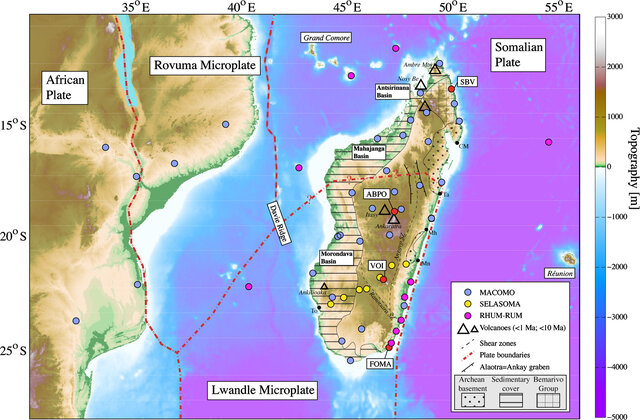
\includegraphics[width=0.5 \linewidth]{./Figures/TopologicMaps/geologyMadagascar.jpeg}
    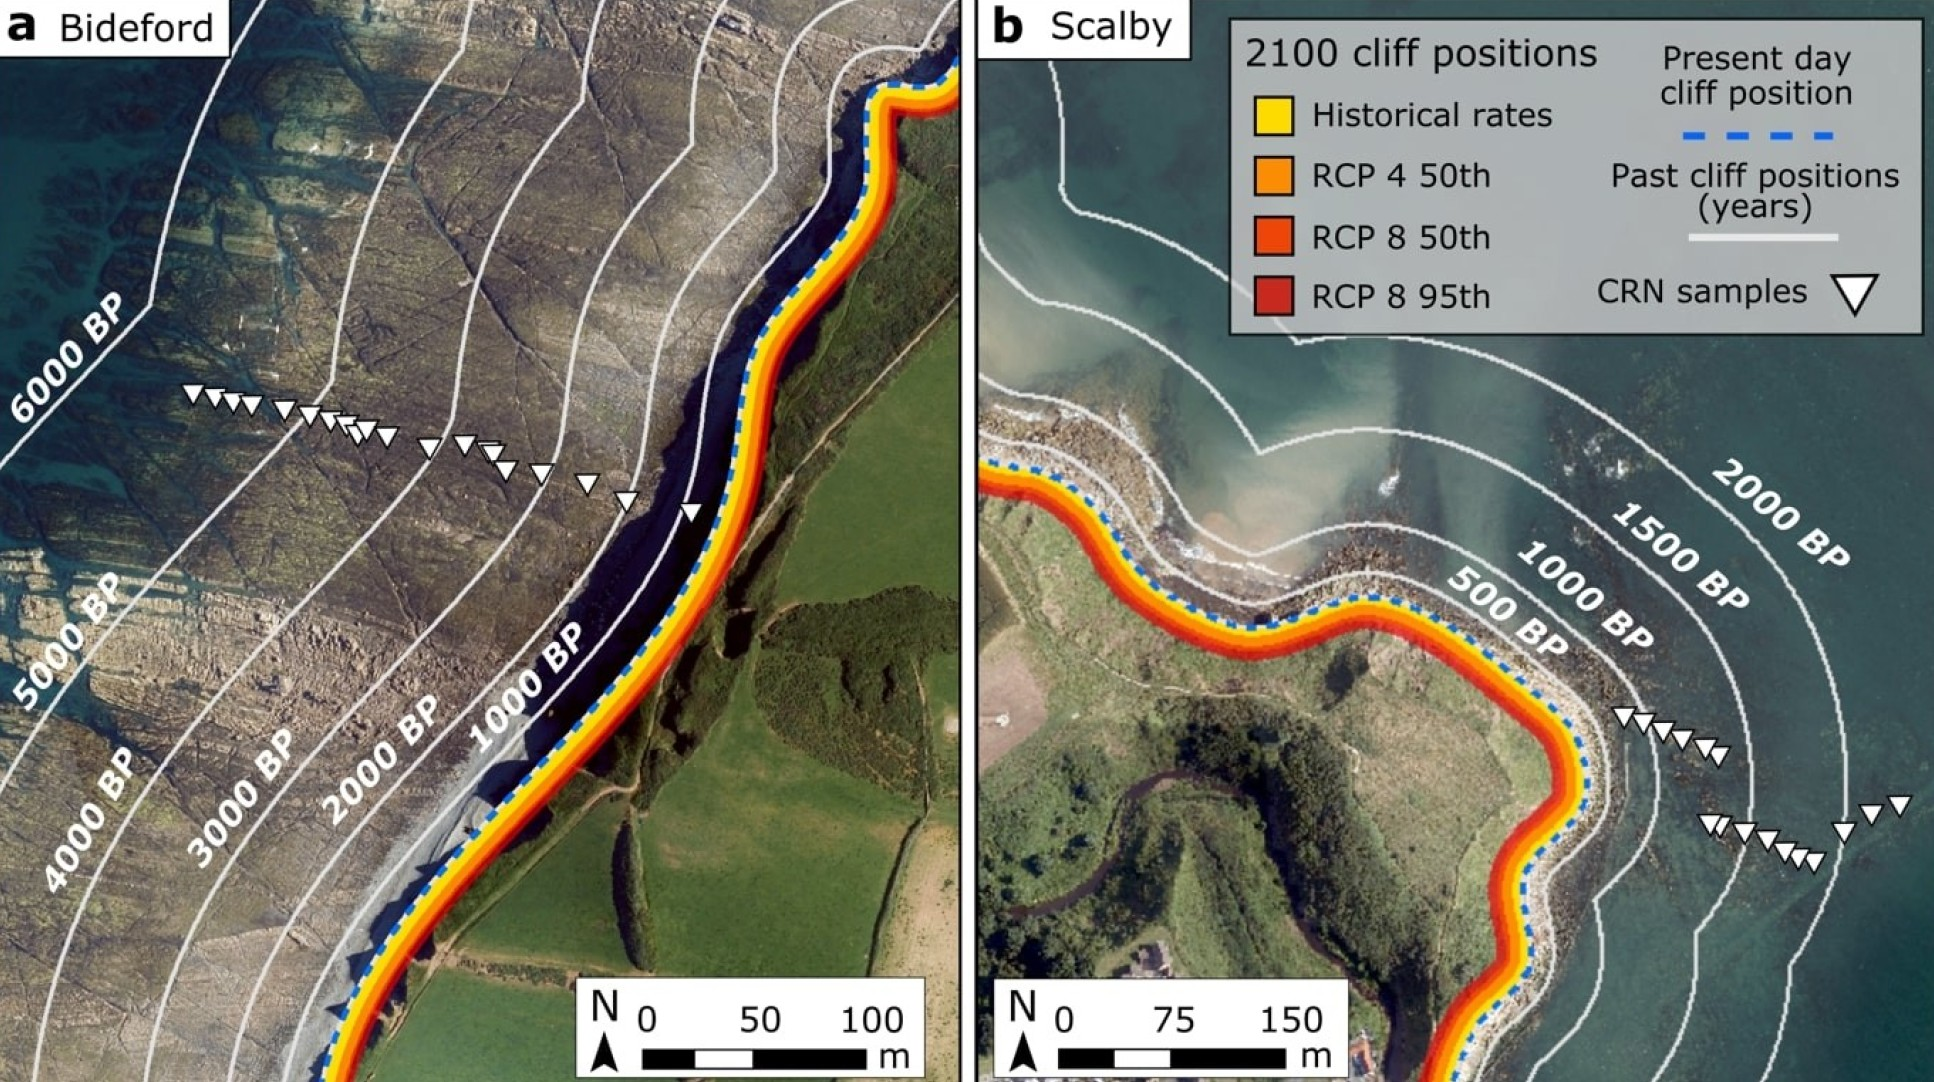
\includegraphics[width=0.5 \linewidth]{./Figures/TopologicMaps/CliffErosionBidefordAndScalby.jpg}
    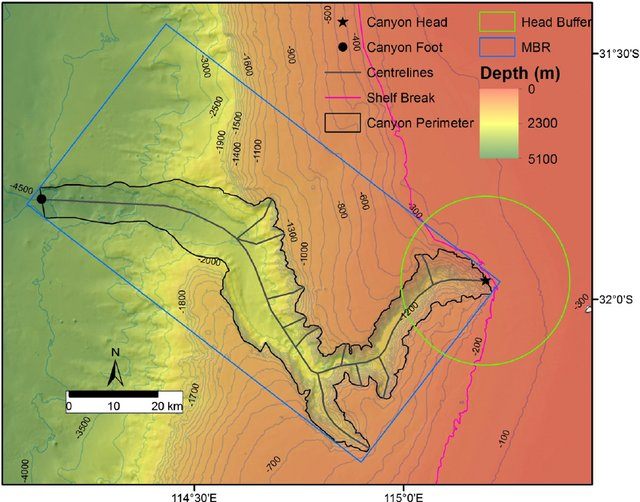
\includegraphics[width=0.5 \linewidth]{./Figures/TopologicMaps/PerthCanyon.jpg}
    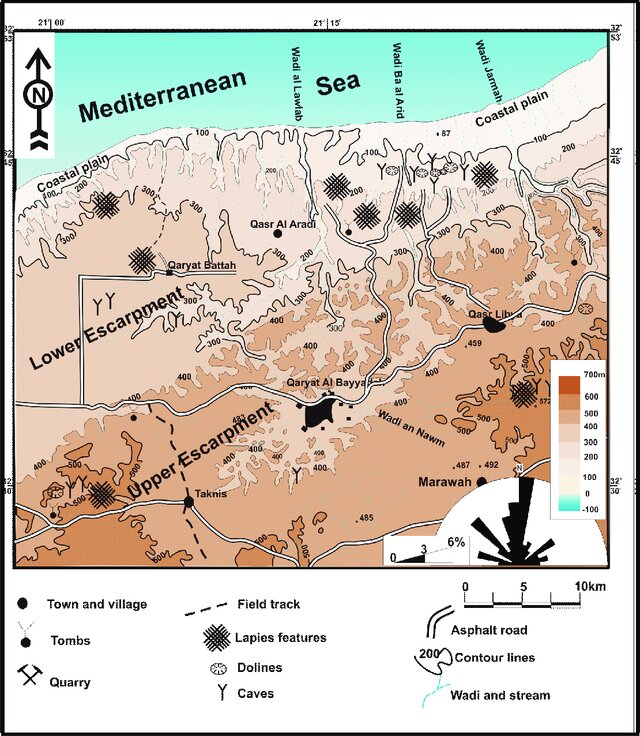
\includegraphics[width=0.5 \linewidth]{./Figures/TopologicMaps/QasrLibya.jpg}
    \caption{Four examples of topographic maps used in earth science. From left to right and top to bottom: Sedimentary distribution other Madagascar island \cite{Pratt2017}, evolution of coastlines at Bideford, UK and Scalby, UK over the last 6000 years and 2000 years respectively (BP = Before Present) \cite{Shadrick2022}, localization of key parameters of Perth Submarine Canyon, Autralia \cite{Huang2014}, and geological features distribution of karstic landscape at Qasr Lybia, Libya \cite{ElAmawy2009}}
    \label{fig:semantic-representation_presentation}
\end{figure}

% Slight introduction
Topographic maps are very useful tools for biologists, geologists or even oceanologists (which would call them "bathymetric charts"). These maps are displayed in 2D but provide 3D information about the altitude (or depth), but can also use symbology to represent the important elements that need to be visible. Map symbols are important in order to extract as much information as possible from a 2D object. In cartography, map symbols are defined as geometric primitives such as points, polylines, polygons, and (more rarely) polyhedrons. These symbols are a simplification of the content of an environment, or an abstraction of the 3D nature of the terrain features as we can see in the examples in \cref{fig:semantic-representation_presentation}. This is useful to understand the relationship between the different features, which may enable to deduce physical rules in the evolution of a terrain. 

% WHo would want it, and why?
In such way, geologists can study the distribution of peaks in a mountain range, the location of soil types in an area, which in turn allow to deduce possible locations of karst networks, for example. Using the same tools, a biologist may interpret the effect of natural or artificial reefs on coastal erosion, or understand more clearly the interactions inside an ecosystem. Oceanologists may also deduce, using the same strategy, the formation of canyons and fans from old river systems. [A REDIRE]

By simplifying the surface details in maps or models, we can concentrate more effectively on gaining a deep understanding of the underlying processes that shape the terrain. This focused understanding allows us to apply the insights we gain to a wide variety of terrain types. Essentially, this approach enables us to generalize our findings and apply them across diverse geographical landscapes, facilitating broader and more versatile applications of our knowledge.

Parallelly, terrain artists most of the time sketch the global shape of the terrain they will model beforehand, such that they can check, before the modeling part, that the consistency and plausibility of the terrain will be valid. Looking at a simplified map before starting the modeling step allows the designer to modify the overall shape of the terrain, at a large scale, before the 3D geometry comes into play, generating too much control points or vertices to be able to deal with.

Starting from an initial configuration or providing conditions on the desired output terrain, the algorithm we propose will let the different terrain features evolve as a multi-agent system in which the user can apply modifications or new constraints on the state of the environment. The resulting configuration is an environment conform to the constraints given by the user over the distribution of features present in the scene.

% Why it does not already exists?
As described in the previous chapter, most terrain generation algorithm use the geometry of an initial terrain surface to iteratively apply changes such as noise-based algorithms or erosion simulation. While the introduction of information about some environment variables or properties of the ground may influence the result of an algorithm, the control of the global shape of the terrain is lost as it treat locally the surface, without knowing which feature a certain point on the surface lies on.

% Personal motivation
The question which led to our solution is the multi-scale user interaction: "Is it possible to provide an interaction mean for terrain generation allowing the user to interact with a small structure like a rock in the same manner as with a large structure like a mountain?". 
In this work, we want the user to be able to have a large scale representation of the terrain in order to generate a landscape that satisfies his needs while keeping the possibility to apply large modifications.
In discussion with robotician users, we realise that we want to create a large landscape that can contain interesting configurations, select a smaller region that may have features in a disposition that fits its requirements and then refine again the given region.
In the optic of generating a large scale terrain in which we could focus the generation effort in a certain region, we wished to be able to see a coarse representation that can be computed quickly.

We aim for our terrain generation method to be versatile enough to handle both terrestrial and aquatic environments. This dual capability would allow the method to be applicable to landscapes above the water level, such as mountains and valleys, as well as to submerged terrains, such as oceanic canyons and coral landscapes.

Because many geographical terms and computer science terms are deceptive cognates, we will try to find middle ground in the naming of our introduced structures to avoid as much as possible any ambiguity between the research fields.
% Because many geographical terms would become ambiguous in computer science terms, in which this thesis lie in, we will translate some vocabulary in a way that may be disapproved by geologists, but we are doing our best to keep it as acceptable for each field as possible.


% \subsection{Nomenclature}
% % Geographical feature/entity -> Semantic Terrain Entity
% A geographical feature, also known as a feature, object, or entity, is a discrete phenomenon located at or near the Earth's surface, relevant in geography and geographic information science. It represents geographic information that can be depicted in maps, geographic information systems (GIS), and other forms of geographic discourse. The term "feature" includes both natural and human-made objects, ranging from tangible items like buildings to intangible concepts like neighborhoods. Features are distinct entities with defined boundaries, differentiating them from continuous geographic masses or processes occurring over time. They can be categorized as natural features, such as ecosystems, biomes, water bodies, and landforms, or artificial features, such as settlements, administrative regions, and engineered constructs. Geographic features are described by characteristics including identity, existence, classification, relationships with other features, location, attributes, and temporal aspects. Information about these features is stored in geographic databases using models like GIS datasets, which organize and represent these features in structured formats.
% % A geographical feature, also referred to as a feature, object, or entity, is a discrete phenomenon located at or near the Earth's surface, relevant in geography and geographic information science. It is an item of geographic information that can be represented in maps, geographic information systems (GIS), remote sensing imagery, statistics, and other forms of geographic discourse. The term "feature" is broad and inclusive, encompassing both natural and human-made objects. It includes tangible items like buildings as well as intangible concepts like neighborhoods. Features are discrete entities with distinct identities and locations, characterized by defined boundaries that differentiate them from other objects, distinguishing them from geographic processes, which occur over time, and geographic masses or fields, which are continuous. In geographic information science, "feature," "object," and "entity" are often used interchangeably, although some formal distinctions exist, such as seeing a feature as an abstraction of a real-world phenomenon. Geographical features can be categorized into natural and artificial types. Natural features include ecosystems, which are communities of organisms interacting with their environments; biomes, which are large areas with ecologically similar communities defined by plant structures, climate, and ecological patterns; water bodies, which are significant accumulations of water like oceans and lakes, either distinct or conceptual in nature; and landforms, which are physical structures such as mountains and valleys defined by surface form, location, and topography. Artificial features encompass settlements, which are human communities ranging from small villages to large cities, including infrastructure like roads and buildings; administrative regions, which are social constructs like states and neighborhoods used for organizational purposes; engineered constructs, which are man-made structures such as highways and airports; and cartographic features, which are abstract map representations, such as grid lines and boundaries, that do not physically exist. Geographic features are represented by descriptors of their characteristics, including identity, existence, kind, relationships, location, attributes, and time. Each feature is unique, often identified by names or codes, and its existence refers to its presence in the real world, including features that are proposed or planned. The kind refers to its classification, such as a building or river, while relationships describe spatial, meronomic (part-whole), and genealogical (parent-child) connections with other features. The location provides a description of where a feature is, including its shape and extent, and attributes describe other characteristics, such as population or size, often expressed as text or numbers. Time relates to the temporal aspects of a feature's characteristics, describing changes over time. Information about features is stored in geographic databases, often using vector data models, including GIS datasets, which help represent these features and their various descriptors in a structured format.

% % Field -> Environmental Attribute
% In geography, the term "field" refers to a continuous spatial phenomenon defined across a region, where each point in that region has a specific value of some variable. Unlike discrete objects, which have distinct boundaries and identities, fields represent variations of phenomena occurring over a continuous space, such as temperature, elevation, or precipitation. Fields can be either scalar or vector quantities: scalar fields represent a single value at every point, like temperature, humidity, or elevation, while vector fields represent quantities with both magnitude and direction, such as wind velocity or ocean currents. Examples of fields in geography include topographic fields, where elevation values are distributed across a landscape; climatic fields, where temperature or precipitation values are mapped over a geographic area; and magnetic fields, which capture the intensity and direction of magnetic forces at various points on the Earth's surface. Fields are often represented mathematically using functions or equations that define how the field's value varies over space, including interpolation or modeling techniques to estimate field values at unsampled locations. In Geographic Information Systems (GIS), fields are typically represented as raster data, where a grid of cells captures the continuous variation of a field across a landscape, with each cell holding a value representing the field's magnitude at that location. Fields are crucial for spatial analysis and modeling, allowing geographers to study patterns and processes that vary continuously across space, such as climate change, land surface modeling, and resource distribution. Thus, in geography, a field is a method of representing continuous spatial phenomena, enabling the analysis of patterns and trends across geographic spaces.

% % Event -> Geological Event
% In philosophy, an "event" is defined as an occurrence or happening that takes place at a specific time and location, characterized by its temporal nature and involvement in change or transition. Unlike static objects, events are dynamic and are often considered fundamental constituents of reality. They typically involve transformations from one state to another, such as a tree falling, and are central to discussions about causality, as they can serve as causes or effects within causal chains. Philosophers debate whether events are basic entities or reducible to other kinds of entities, like properties of objects or states of affairs. They also explore how events are individuated and identified, what distinguishes one event from another, and how events relate to objects. Linguistic and logical analyses focus on how events are described in language, often through verbs and predicates, and how they relate to entities involved. Various philosophical theories, such as process philosophy, emphasize events over static entities, offering different frameworks for understanding the nature of events and their role in the structure of reality. Overall, events are crucial for understanding change, causality, and our perception of the world.

% % Visualization

% \subsection{Features on field experts maps}
% - ... 
% \subsection{Topographic/Planimetric maps}
% - ... 

% \subsection{Analogy}
% - Compare our nomenclature with introduction \\
% - ... 

\section{State of the art}
\label{sec:semantic-representation_related-works}

\subsection{Vector modeling}
...
\subsubsection{Implicit modeling}
...
\subsubsection{Diffusion models}
...

\subsection{Ecosystems simulation}
...
\subsubsection{Environment modeling}
...
\subsubsection{Individual process}
...
\subsubsection{Multiple entity simulation process}
...
\subsubsection{Cellular automata}
...

Procedural terrain generation has been heavily studied for the last 40 years \cite{Galin2019}. Researches in this topic try to find new solutions to compromise between realism, user control and efficiency \cite{Gain2009}. Using fractal noise parametrized to resemble real landscape has been an important first step \cite{Musgrave1989} as it's a fast and light solution to generate procedurally the appearance of mountains. The lack of user control pushed newer works toward the use of controlled noise by including real DEM in the process through learning \cite{Kapp2020, Brosz2007}, while the rise of deep learning technologies gave higher control to the user through sketches \cite{Guerin2017, Talgorn2018}.

All the algorithms aim to reproduce plausible relief in terrestrial landscapes, mostly limited to alpine landscapes, but a lack of research can be found in almost all other biomes \cite{Smelik2014}. Underwater landscapes generation, for example, has been almost completely absent from literature for many reasons: the difficulty of accessing the area, the lack of visibility under water and the complex physics of underwater geology and biology make the algorithms adapted for this environment scarce. 

While stochastic noise can be sufficient to model coarsely the ocean floor \cite{Mareschal1989}, this process won't cover areas with the biggest biomass, near shallower waters such as near coasts and islands. These areas, that represent a very small portion of the oceanic surface, are much more complex as many interactions between biolife, air and water are in action.

Due to the impossibility to observe the large-scale and the small-scale of underwater environments, some works related to geology model large structures like the profile shape of the coral reef \cite{Bosscher1992}, simulate its surface growth \cite{Li2021}, or use procedural algorithms for single coral colonies' growth simulation \cite{Abela2015}. We however don't have a mix of the different scales, and neither methods take into account the environment such as the topography or the interaction of different terrain features. This is mainly due to the fact that the evolution time for each scale varies from a span of weeks to thousands of years.

Recent works have been presenting "feature tools" to correct landscapes from unaccurate DEM (2.5D) using vector-based features that modifies the geometry of the ground and water bodies to fit thir respective 2D satellite images, by explicitely defining the position of natural features like rivers and mountains \cite{Ketabchi2016}. Visible 3D features like vegetation and buildings can also be added in the final result as meshes affected to a single point. This leads to sketch-based applications where features are represented like topographic maps. This solution allows for the manipulation of an existing terrain, guided by a real-world satellite image, but lacks the possibility to completely generate an unseen landscape or for the terrain features to interact between them. Feature tools have been proposed to generate terrains from scratch \cite{Smelik2010a}, but usually require to define in advance the interactions between each feature like a automatically displaying a bridge when a river crosses a road.

In an ecosystem, every element within the system has an impact on its surroundings, and accurately simulating physical properties like shading, heat, and humidity can require immense computational power. To address this, instead of simulating these properties individually for each object, they can be represented as scalar fields that span the entire scene. These scalar fields, which may represent temperature, humidity, or occlusion, are locally influenced by nearby objects and terrain features, such as trees casting shadows or buildings radiating heat. This approach, as described in \cite{Grosbellet2016, Guerin2016a}, allows for the environment's physical properties to be computed in a more efficient manner. By simplifying the complex interactions into these localized scalar fields, they called environmental objects, their method provides a scalable system that can handle large and detailed scenes. This system effectively renders scene details, such as snow accumulation or leaf distribution, in a way that is visually plausible, ensuring realistic results without the need for exhaustive simulations. 
%In a similar way, other works represent the wind flow as a composition of local vector fields \cite{Wejchert1991}, avoiding complex fluid simulation while providing user control in a lightweight model. We extend these works by incorporating a time-evolution system such that the scene can be dynamic.
In a similar approach, parallely Wejchert and Haumann \cite{Wejchert1991} and Sims \cite{Sims1990} represent wind flow as a composition of local vector fields, known as "flow primitives", which can be combined to simulate complex fluid behavior. This method simplifies the computation by avoiding full fluid simulations, instead offering a lightweight model that allows for intuitive user control over the flow dynamics.
By combining these approaches, we can create dynamic ecosystems where environmental effects and fluid flows interact in a plausible manner, while requiring a low computation effort and preserving a high user control.


\section{Description of the method}
\label{sec:semantic-representation_pipeline}

In this section, we present the pipeline and processes that underpin our method. Our approach introduces the concept of \glosses{EnvObj}, simplified terrain features that interact with their surroundings to simulate complex ecosystem dynamics. These \glosses{EnvObj}, which can represent natural features such as trees, rivers, or rocks, influence and are influenced by scalar fields like temperature, humidity, and elevation. The method is structured into several key phases: initialization, where the foundational elements of the terrain and \glosses{EnvObj} are set up; an iterative generation process, where these \glosses{EnvObj} are instantiated and interact with their environment; and finally, the production of a sparse representation of the scene's features. This section details each of these phases, explaining how the system dynamically adapts to user input and environmental changes.

\subsection{Pipeline}

\begin{figure*}
    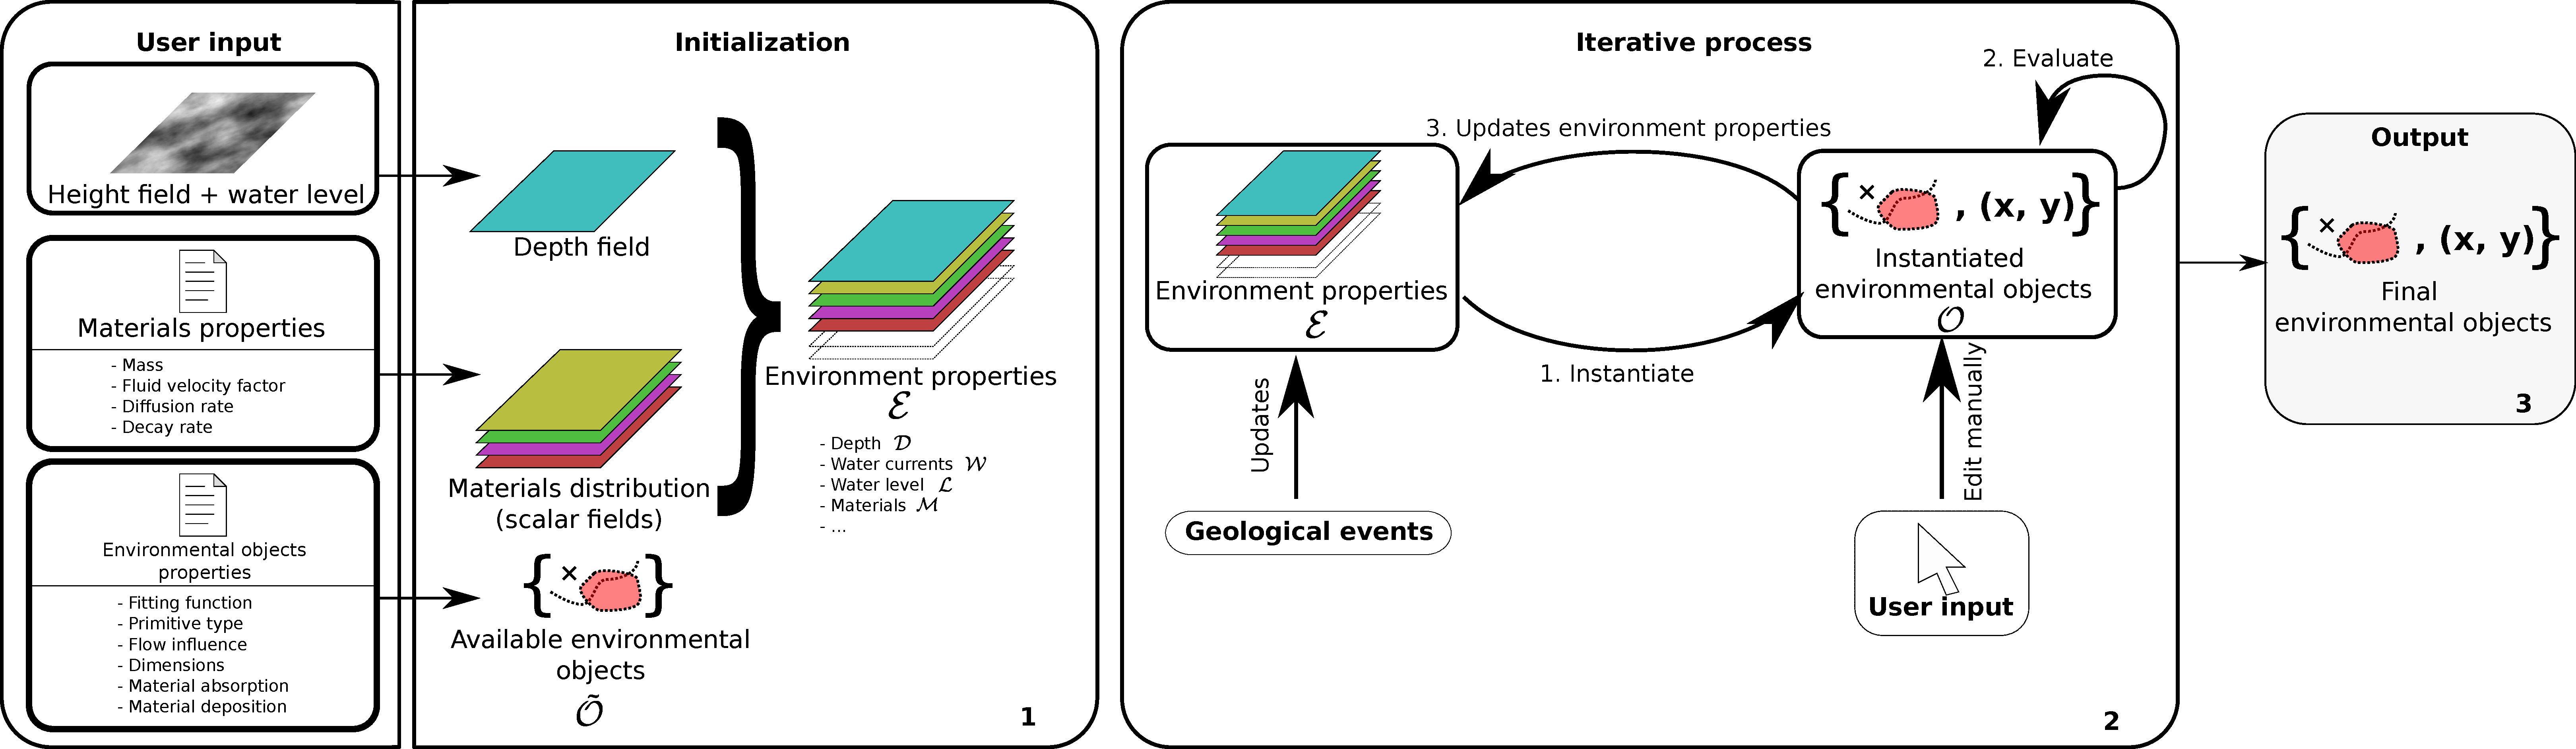
\includegraphics{Figures/pipeline.pdf}
    \caption{Overview of the pipeline of the method. The user provides as input an initial height field and sets the water level, as well as a definition of the \glosses{EnvMat} properties and \glosses{EnvObj} properties that will be used in the iterative process. These inputs are initialized as an initial set of \glosses{EnvObj} and scalar fields that represents the \glosses{EnvVal}. In the iterative loop, new \glosses{EnvObj} are instantiated using the current state of the environment at their optimal position. The existing \glosses{EnvObj} in the terrain reevaluate their \gloss{FitnessFunc} to grow or die and update the \glosses{EnvVal} locally. At each iteration, \glosses{GeoEvent} can update the \glosses{EnvVal}, while the user can interact directly with the \glosses{EnvObj}. The result of the whole process is a set of \glosses{EnvObj} which is a sparse representation of the features of the scene. }
    \label{fig:semantic-representation_pipeline}
\end{figure*}

\subsubsection{Initialization}

The generation of the terrain is initialized using an initial height field $h$ and an initial water level $\Wlevel$. 
During this chapter we will include many features depending on altitude or depth, so we will use the shorthand notations $\height = h - \Wlevel$ and $\depth = -\height$. The height field provides variation on the altitude, which can influence the generation process of the scene.

The list of available \glosses{EnvObj} $\availableObjects$, representing the different features that can be present in the scene, are provided with their properties: type, size, \glosses{GenRule} and effects on the \glosses{EnvVal} (\cref{sec:semantic-representation_environmental-objects}). A target list of \glosses{EnvObj} $\targetObjects$ can be defined to control the final result of the generation.

Finally, different \glosses{EnvMat} are defined with their properties such as diffusion speed, mass, decay rate and influence from the water currents. An initial environment configuration resulting from the initial height field $\height$ and water level $\Wlevel$, the \glosses{EnvMat} distribution $\material$ (represented as scalar fields $\material: \R^2 \to \R$) and water currents $\Water$ (as a vector field $\Water: \R^2 \to \R^2$) will be used by the \glosses{EnvObj} of the scene to simulate their growth and spawn at the most probable position. The \glosses{EnvVal} are noted $\environment = (\depth, \Water, \Wlevel, \material)$ (\cref{sec:semantic-representation_communication}).

The definition of \glosses{EnvObj}' properties and \glosses{EnvVal} is done with field experts, providing the pertinent parameters required to model the evolution of the terrain features using expert knowledge (\cref{sec:semantic-representation_biology}). 

The generation phase starts with an initial set of \glosses{EnvObj} present in the scene, which can optionally be pre-filled.

\subsubsection{Generation process} 

%- Main loop
Once the initialization phase is done, the generation begins. The generation process is incremental and its main loop is composed of two different steps: the instantiation of new \glosses{EnvObj} then the update of the environment. This loop is repeated until the user is satisfied with the look of his environment or following rules like a number of features threshold or a targeted list of \glosses{EnvObj} as described in the layout planner defined in \citep{Tutenel2009}.


\subsubsubsection{Instantiation}
% - Object instantiation
At each iteration, new \glosses{EnvObj} can be created at their most fitting locations if possible. The \glosses{GenRule} provided in the initialization phase are used to find an optimal position from stochastic sampling (\cref{sec:semantic-representation_generation-rules}). 
All \glosses{EnvObj} are evaluating their state analytically using a \gloss{FitnessFunc} and a \gloss{FittingFunc} provided as input (\cref{sec:semantic-representation_generation-rules}).

\subsubsubsection{Environment update}
% Once the new objects are instantiated, the process can continue.
% - Environment update
Once the instantiation step is done, the \glosses{EnvVal} are updated by each \gloss{EnvObj} through \glosses{EnvModif}, which depose and absorb some of the \glosses{EnvMat} $\material$ (\cref{sec:semantic-representation_materials}) while modifying the water currents $\Water$ (\cref{sec:semantic-representation_water-currents}) and the height field $\height$ around them. Finally, water currents and terrain slope displace \glosses{EnvMat} of the terrain until reaching a dynamic equilibrium in the environment at each iteration.

% We consider the water currents to be a steady-state flow, allowing us to remove the variation from time in the flow equations.
% The water currents are updated locally by each \gloss{EnvObj} using an analytical form $W^*(\p) = W(\p) + \omega(\p)$.
During the generation process, the user can alter directly the distribution and shapes of the \glosses{EnvObj} (\cref{sec:semantic-representation_manual-interaction}) and perturb the generation process by planning \glosses{GeoEvent} that have impacts on the \glosses{EnvVal} (\cref{sec:semantic-representation_events}).


\subsubsection{Output}
% - Output result
The output of our system is a set of \glosses{EnvObj} disposed in the plane. We do not provide the 3D representation of the \glosses{EnvObj} in this chapter, letting the user define the rendering method. The figures used in the chapter use a mix of implicit surfaces and triangular meshes.

\subsection{\Glosses{EnvObj} $\objects$}
\label{sec:semantic-representation_environmental-objects}
A geographical feature, also called object or entity, is defined as a discrete phenomenon located at or near the Earth's surface, relevant in geography and geographic information science (GIScience). It represents geographic information that can be depicted in maps, geographic information systems (GIS), and other forms of geographic media. This term includes both natural and human-made objects, ranging from tangible items like buildings or trees to intangible concepts like neighborhoods or savana. Features are distinct entities with defined boundaries, differentiating them from continuous geographic masses or processes occurring over time. They can be categorized as natural features, such as ecosystems, biomes, water bodies, and landforms, or artificial features, such as settlements, administrative regions, and engineered constructs. Geographic features are described by characteristics including identity, existence, classification, relationships with other features, location, attributes, and temporal aspects. Information about these features is stored in geographic databases using models like GIS datasets, which organize and represent these features in structured formats. As the term "feature" is overused in computer science, we will use the term \gloss{EnvObj} in this work.

Each \gloss{EnvObj} is shaped with a simple geometric shape called a "skeleton" that defines where it is located and how it fits into the environment. The \gloss{Skeleton} can either be, as used in cartography, a point, a curve or a region. We will then refer to our \glosses{EnvObj} as point-based, curve-based or region-based, respectively.  
These \glosses{EnvObj} interact with the environment $\environment$ by changing local conditions using the \glosses{EnvModif}. For example, the presence of a river might increase the moisture in the surrounding area, while a mountain might induce more rockiness in the soil composition. They can also absorb changes from the environment, such as a forest taking in humidity from the air.
The placement of \gloss{EnvObj} is determined by a \gloss{FitnessFunc} $\fitnessFunc$, which evaluates how suitable a location is based on the \glosses{EnvVal}. Once a suitable location is found, the \gloss{FittingFunc} optimizes the shape and position of the entity to fit as best as possible into the environment $\fittingFunc$.

%This approach allows us to "spawn" new entities based on rough altitude estimates, ensuring that their placement is contextually appropriate while deferring the detailed computation of their final shape to a later stage, if required by the user.
% The coarse height function thus acts as a middle between the semantic modeling of terrain and the precise 3D modeling. It provides enough information to make informed decisions about \glosses{EnvObj} placement and \glosses{EnvMat} while preserving the flexibility to integrate more detailed modeling techniques. This method ensures that the terrain generation remains interactive and scalable, allowing for the dynamic and realistic placement of entities in complex landscapes without being tied to the immediate computation of detailed topography.

% \Glosses{EnvObj} are rule-based objects following rules depending on their local environment for evaluation their state in their life cycle. We can see them as a life form in the way that they are created and eroded with time. During their lifetime, they influence their local environment by depositing and absorbing \glosses{EnvMat} around them and influencing the water currents. The environment objects are described spatially as a single point, a parametric curve or a region.


\subsection{\Glosses{EnvVal} $\environment$}
\label{sec:semantic-representation_communication}

In geography, a "field" refers to a continuous spatial phenomenon across a region where each point has a specific value of a variable, unlike discrete objects with distinct boundaries. Fields can be scalar, representing a single value at every point (like temperature or elevation), or vector, representing quantities with magnitude and direction (like wind velocity). Examples include topographic fields for elevation, climatic fields for temperature or precipitation, and magnetic fields for magnetic forces. Because of the ambiguous nature of the term "field" with mathematics and computer science, we will define the geographic fields as \gloss{EnvVal}.

In an ecosystem simulation, each actor of the ecosystem has an impact on all other actors, which results in an exponentially growing computation effort as the number of elements of the terrain increase. We avoid this problem by considering the \glosses{EnvVal} as a proxy to allow any \gloss{EnvObj} to interact with any other one. Each of the \gloss{EnvObj} have a local impact on the \glosses{EnvVal} without knowledge of neighboring \glosses{EnvObj}. This modification of the \glosses{EnvVal} are presented as the effect of \glosses{EnvModif} defined for each \gloss{EnvObj}. % can be due to an absorption and deposition of some material $\material$ or an influence on the water currents.

In this work, we have integrated vector \glosses{EnvVal} (e.g., water currents $\Water$) and scalar \glosses{EnvVal} (e.g., altitude $\height$, water level $\Wlevel$, and various material properties $\material$) under the unified term "environment," denoted as $\environment = \left( \height, \Water, \Wlevel, \material \right)$. The \glosses{EnvMat} represent abstract quantities such as the availability of sand, salt, moisture, or rocks at each point. It is important to emphasize that these materials are not to be visualized as physical layers stacked on the terrain surface. Instead, they should be understood as conceptual resource distributions that influence the environment and the behavior of \glosses{EnvObj}, rather than as something directly observable in the scene.

\subsubsection{\Glosses{EnvModif} $\environmentModif$}
The environment determine if a \gloss{EnvObj} does belong at a certain position. When a \gloss{EnvObj} is placed, its surrounding \glosses{EnvVal} can be affected though \glosses{EnvModif} noted $\environmentModif = (\heightModif, \waterModif, \nothing, \materialModif)$ defining a change of height $\heightModif$, changes in the water currents $\waterModif$ and \gloss{EnvMat} alteration $\materialModif$. 

\Glosses{EnvObj} are subject to altitude conditions. However, to maintain a clear distinction between semantic modeling and 3D modeling, we do not compute the exact physical shape or detailed height field of each \gloss{EnvObj}. Instead, we define a \gloss{CoarseHeight}, a parametric representation derived from the \gloss{Skeleton} to provide a rough estimate of the changes in elevation around it. This simplified model of how the \gloss{EnvObj} influences the surrounding terrain's altitude allows us to cheaply evaluate the potential presence of new entities that have altitude-dependent conditions without the need to perform expensive computations to generate a detailed height map of the entire terrain. 

Altering the vector field of the water currents $\Water$ is done by the composition of the effect $\waterModif$ of each object at a position $\p$ as introduced in \citep{Wejchert1991}, while we use the formulation of Kelvinlets \cite{DeGoes2017} in the computation of effect of each \gloss{EnvObj}.

Each \gloss{EnvObj} has intrinsic \glosses{EnvMat} that can be seen as "spreading" and "absorbed" around its skeleton over time. A coral reef may produce coral polyps and at the same time reduce the water currents. It grows thanks to the deposition of limestone from coral colonies. In our model, the colonies affect the \glosses{EnvVal} through the deposition of \gloss{EnvMat} $\materialModif_\text{limestone}$, which in turn, is absorbed by the coral reef, without a direct exchange between the two \glosses{EnvObj}.

The alteration of a scalar \gloss{EnvVal} is done by adding or removing some amount around the \gloss{Skeleton} of the \gloss{EnvObj} and diffusing it in the space, influenced by the water currents. We consider the system to be \gloss{SteadyState}, garantied by the introduction of a decay rate $\decay > 0$ in the computation of the diffusion and advection.



\section{Placement of \glosses{EnvObj} in an environment}
\label{sec:semantic-representation_generation-rules}

At each iteration of our algorithm, we want our \glosses{EnvObj} to be at plausible positions. We do not guaranty a temporal continuity between iterations as in \citep{Ecormier-Nocca2021}, so the objective is to add new \gloss{EnvObj} in order to satisfy the users wishes, while conserving the plausibility of the scene. Rather than "forming" these \glosses{EnvObj}, our method "reveals" them, much like a paleontologist uncovers fossils during an excavation. A paleontologist does not dig randomly across the Earth to find fossils; instead, they analyze the geological context to identify the most likely locations. Similarly, our method observes the environment and estimates where certain elements are likely to exist. For example, in hydrology, if a river appears to originate from nowhere, it might suggest the presence of a karstic river system upstream. In urban planning, if many roads converge at a certain point, it is reasonable to expect that a city is located there. This approach ensures that Semantic Terrain Entities are revealed in positions that are contextually appropriate and coherent within the landscape.

We will follow the same intuition using a \gloss{FitnessFunc} for each of the \gloss{EnvObj} that may be spawn in the terrain. The \gloss{FitnessFunc} defined $\fitnessFunc: \environment \to \R$ provides a score indicating how well the \gloss{EnvObj} may fit in this position. Evaluating this function at multiple position results in an approximation of the fitness map of the entity. Once the most probable position is found, we can find the most plausible shape of the \gloss{EnvObj} using the \gloss{FittingFunc} $\fittingFunc$.

For this task, we place a new elements required at the most plausible position using the analysis of the \gloss{FitnessFunc} of each \gloss{EnvObj}. We know that each \gloss{EnvObj} will modify the environment surrounding, which may make previously instantiated \glosses{EnvObj} unfitted. Knowing this,the goal is to add the new element at the position that will change the least the stability of the system. 

Genetic algorithms or Depth First Search algorithms could be used to try many possibilities until a local or global minimum could be found, but this would require a large processing power. Naive genetic algorithms would place a \gloss{EnvObj} at a certain position at each iteration and evaluate the stability of the environment, repreating this operation while varying slightly the position of the \glosses{EnvObj} or the type of \gloss{EnvObj} instantiated at each iteration, resulting in way too much computation to stay interactive. The Depth First Seach algorithms would require to compute all the possible combinations of \glosses{EnvObj} and positions which, given the fact that we want a continuous position in order to work multi-scale, would require to compute an incredibly high amount of possible configurations in order to find a plausible situation, on average. We will work with an evolutionary algorithm to find a compromise between fast computation and a satisfying result.

Our placing algorithm is done in two steps: first, it identifies the global location where a \gloss{EnvObj} best fits within the environment $\environment$ using its \gloss{FitnessFunc} $\fitnessFunc$, which evaluates the suitability of each point $\p$ based on the \glosses{EnvVal} $\environment_p$, including factors such as altitude $\height(\p)$, water current velocity and direction $\Water(\p)$, water level $\Wlevel(\p)$, and the availability of \gloss{EnvMat} $\material(\p)$. Second, once the most suitable location is identified, the algorithm determines the most plausible shape of the \gloss{EnvObj} using the \gloss{FittingFunc} $\fittingFunc$.

To ease the reading the functions $\fitnessFunc(\environment(\p))$ and $\fittingFunc(\environment(\p))$ with $\environment(\p)$ the \glosses{EnvVal} at the point $\p$ of the terrain are simplified to $\fitnessFunc(\p)$ and $\fittingFunc(\p)$ respectively.

% Our placing algorithm is done in two steps: first we estimate at which global location the \gloss{EnvObj} fits the most given an environment $\environment$ using its \gloss{FitnessFunc} $\fitnessFunc$, secondly we estimate the shape of the skeleton of this \gloss{EnvObj} should take given a \gloss{FittingFunc} $\fittingFunc$.

% \Glosses{GenRule} provides, for each \gloss{EnvObj}, a \gloss{FitnessFunc} $\fitnessFunc$ defining the most probable location for an \gloss{EnvObj} to be found. \Glosses{FitnessFunc}' parameters contains, for every point $\p$, the \glosses{EnvVal} $\environment_p$ (the altitude $\height(\p)$, the velocity and direction of the water currents $\Water(\p)$, the water level $\Wlevel(\p)$ and the amount of each \gloss{EnvMat} available $\material(\p)$).

\subsection{\Gloss{FitnessFunc} $\fitnessFunc$}
"Darwinian fitness" refers to an organism's ability to survive and reproduce in its environment. It is a measure of how well-suited an organism is to its surroundings, and those with higher fitness are more likely to pass on their genes to the next generation. In a similar vein, the \gloss{FitnessFunc} of a \gloss{EnvObj} evaluates its suitability at a location in the terrain, extending the meaning to living features like forests and corals and non-living elements such as rivers, mountains, karsts, etc.

The fitness function is constructed by evaluating several environmental variables at a given location $\p$. These include altitude ($\height(\p)$) and its gradient ($\nabla \height(\p)$), the availability and gradient of various materials ($\material_i(\p)$ and $\nabla \material_i(\p)$), water current characteristics ($\Water(\p)$), and water level ($\Wlevel(\p)$). Altitude and its gradient can influence the placement of objects like rivers, which may prefer lower elevations, or forests, which might thrive on slopes. Each material, such as limestone, sand, or clay, is considered separately, and their availability and gradients at a location are crucial for determining the suitability of different \glosses{EnvObj}, such as a coral reef requiring specific substrates. The velocity and direction of water currents are essential for placing aquatic features or determining where erosion might occur, while the proximity to water influences the likelihood of placing wetlands, lakes, or other hydrological features.

These environmental variables are typically combined in the fitness function, often expressed as a weighted sum, but not restricted to this form:

\begin{align*}
    \fitnessFunc(\p) = w_1 \cdot \height(\p) + w_2 \cdot \nabla \height(\p) + \sum_{i} \left( w_{3,i} \cdot \material_i(\p) + w_{4,i} \cdot \nabla \material_i(\p) \right) + w_5 \cdot \Water(\p) + w_6 \cdot \Wlevel(\p)
\end{align*}

Here, $w_1, w_2, w_{3,i}, w_{4,i}, w_5, w_6$ are weights that reflect the relative importance of each factor for the specific \gloss{EnvObj} being considered.

Different types of \glosses{EnvObj} require different criteria for their fitness evaluation. For example, a river might prioritize lower altitude and proximity to water currents, while a forest might prioritize higher altitude and specific material availability. The flexibility of the fitness function allows it to be customized for each \gloss{EnvObj}, ensuring that the generated terrain remains coherent and realistic.

\subsection{\Gloss{FittingFunc} $\fittingFunc$}
The seed point of a spawning \gloss{EnvObj} is defined at the point $\p$ satisfying $\arg \max_\p \fitnessFunc(\p) $.
% a stochastic sampling of the plane. We propose different optimization means to find the optimal fitting position, depending on the \gloss{EnvObj} shape.

\subsubsection{Point-based \gloss{Skeleton}}
The spawning position of a punctual \gloss{EnvObj} is found at the local maxima of the \gloss{FittingFunc} from the seed point. While the \gloss{FittingFunc} doesn't have to be identical to the \gloss{FitnessFunc}, we usually use $\fittingFunc = \fitnessFunc$ for point-based \glosses{EnvObj}. If the two functions are different, the optimisation process simply follows the field's gradient $\nabla \fittingFunc$ until the local maxima is reached.

\subsubsection{Curve-based \gloss{Skeleton}}
% A curve can have different \glosses{GenRule}, making the definition of the functions easier depending if the \gloss{EnvObj}'s \gloss{Skeleton} has a notion of direction. It can either:
% \begin{itemize}
%     \item follow the gradient of the \gloss{FittingFunc} $\nabla \fittingFunc$, useful when the direction of the \gloss{Skeleton} has an importance like a river that has to run downhill,
%     % \item follow the isocontour $\nabla \fittingFunc^\perp$, [WAIT, IS THAT NEEDED?]
%     \item or optimize the energy of the function over its curve, like a coral reef that has to cover as much coral colonies as possible. % follow the heat points.
% \end{itemize}

% \subsubsubsection{Following the gradient}
% Following the gradient of the \gloss{FittingFunc} $\nabla \fittingFunc$ is done by extending a curve from the seed point towards $\nabla \fittingFunc$ until reaching a local maximum while also following $-\nabla \fittingFunc$ until finding a local minimum. We stop the building process when our curve reaches a length limit $\Length$. 

% This \gloss{FittingFunc} strategy is efficient to describe rivers as we can set $\fittingFunc(\p) = \height(\p)$ to force it to always run downstream. 

% \subsubsubsection{Energy optimization}
The skeleton of a curve-based \gloss{EnvObj} is determined by the shape that fits the most given the environment it is added to. 
Using a modified version the Active Contours algorithm \cite{Kass1988}, we can minimize the energy $\energy$ for the parametric curve $\curve$ given $\energy(\curve) = \Einternal + \Eexternal + \Eshape + \Egradient$ with  
\begin{align}
    \label{eq:internal-energy-equation}
    \Einternal &= \Ainternal \left( \int_{\curve}{ \norm{\curve'(s)}^2 \, ds} + \int_{\curve}{ \norm{\curve''(s)}^2 \, ds}  \right) \\
    \Eexternal &= \Aexternal \int_{\curve}{ \fittingFunc(\curve(s)) \, ds } \\
    \Eshape    &= \Ashape \left( \Length - \int_{\curve}{ \, ds } \right)^2 \\
    \Egradient &= \Agradient \int_{C}{ \dot{C'(s)}{\Delta \fittingFunc(C(s))} \, ds }
\end{align}
In this configuration, $\Einternal$ induce a smooth continuity of the curve by reducing the spacing of each point while reducing the curvature. Another energy, $\Eexternal$ integrate the \gloss{FittingFunc} over the curve, often seen as an attractor of the points, that tries to descent the gradient to find local minima. At the same time, $\Eshape$ apply constraints on the curve shape, which, in this case, is to target a specific length $\Length$. As such, the curve search for an optimized shape given constraints in $\Eshape$ for minimizing $\Eexternal$. We introduced a new term $\Egradient$ in the energy computation that push the points of the curve in the direction of the slope of the \gloss{FittingFunc}, also providing an orientation for the curve.

If a steep coast can be found where the terrain slope is important near the water level, we can define $\fittingFunc = \abs{\height + 1} / \norm{\Delta \height}$, but no orientation is needed, thus we set $\Agradient = 0$. In this case, the curve will follow a path at the water level and spread its extremities over areas with a steep slope. A river may also be symbolized as a parametric curve, but we need to add information about the direction and magnitude of the slope.  As such, we can use $\fittingFunc = \height$ which forces the direction of the curve to fit with the terrain slope. The introduction of the gradient component provides also an orientation to shapes.

\subsubsubsection{Internal energy}
The internal energy, already introduced in \citep{Kass1988} is composed of two components imposing penalities on the local properties of the points of the curve. The first derivative forces the points along the curve to be evenly spaced by minimizing the curve tension, while the second derivative restrict it from forming sharp corners. As our aim is to represent natural elements, we rarely find sharp elements and thus, keep the original definition from the Snake formulation.

\subsubsubsection{External energy}
The external energy is also present in the original work. Using an external scalar field, each point of the curve is forced to follow the steepest slope of the field. The external field can be seen as an attractor for the curve.

\subsubsubsection{Shape energy}
We introduced the shape energy, an energy defined on the whole curve to apply constraints on its final shape. As many natural features have a given dimension, we may add a constraint on the lenght of the \gloss{Skeleton}. 

\subsubsubsection{Gradient energy}
In our application, having information about the orientation of \glosses{EnvObj} may be essential. For this purpose, we introduced a gradient energy component in the formulation. The equation impose that the direction of the curve at any point should be directed towards the gradient of the scalar field. As the external energy pushes points toward the lowest point of the scalar field, the gradient field restrict the gradient descent for the global curve into a specific way, which may feel more natural.

During the optimization process, the gradient of the scalar field is already evaluated by the external energy optimization, so the addition of the gradient component is almost free.

% \subsubsubsection{Position constraint}
% As the curve minimize its energy, it may fly far away from the initial seed point. We added a last constraint about the positioning of the curve such that the distance between t

% The internal energy $\Einternal$ force the shape continuity while the shape energy $\Eshape$ force the shape into a specific target length $\Length$, and finally $\Eimage$ that use the definition of the \gloss{FittingFunc} to attract the points of the curve toward a local minimum.

% While the first two possibilities are trivial, the later can also be optimized using the Active Contours algorithm by optimizing the energy $\energy = \Einternal + \Eshape$ with \eqref{eq:internal-energy-equation}. We applied a length constraint on the curves : 
% \begin{align*}
%     \Eshape = \left( \Length - \length \right)^2
% \end{align*}
% with $\length$ the curve's length and $\Length$ the target length. This algorithm is sensible to the initial shape of the curve, so we start with a straight line following the isolevel at the seed point.

\subsubsection{Region-based \gloss{Skeleton}}

Region-based \glosses{EnvObj} follows the same process than curve-based \glosses{EnvObj} to define their \gloss{Skeleton}, at the exception of the gradient energy $\Egradient$ which have null value on closed shapes. 

The resulting energy $\energy$ to minimize for a closed region whose borders are defined by the curve $\curve$ can then be expressed as $\energy(\curve) = \Einternal + \Eexternal + \Eshape$.

The internal energy is expressed identically as for curve-based \glosses{EnvObj}. The extenal energy however, has to be modified to take into account the interior of the region instead of only the borders. We will use the idea of the Chan-Vese algorithm, differentiating the energy value for the inside $\domain$ and the borders $\curve$ of the region \cite{Chan2001, Getreuer2012}.

By adding a factor for the inside $\lambda_1$ and a factor for the borders $\lambda_2$, we can add weight depending on the required optimization. We can then define the external energy component $\Eexternal$ as:
\begin{align}
    \Eexternal = \lambda_1 \int_{\domain}{ \fittingFunc(s) \, ds } + \lambda_2 \int_{\curve}{ \fittingFunc(\curve(s)) \, ds }
\end{align}
We see that the definition of the energy formulation of the curve-based \glosses{EnvObj} is a specialization of the region-based, with $\lambda_1 = 0$ and $\lambda_2 = \Aexternal$

The use of external forces on the \gloss{Skeleton} can be useful as some landscape features are easier to define by what they contain, while other by what they separate. For example, a lagoon is formed by coral reefs surrounding it, while a forest is formed by the climatic conditions inside it that are propice for trees. A lagoon may then be defined with $\lambda_1 = 0$ and $\fittingFunc_{\text{lagoon}} = -\material_{\text{coral limestone}}$ while a forest sets $\lambda_2 = 0$ and $\fittingFunc_{\text{forest}} = -\material_{\text{humidity}} + \material_{\text{shade}} + \abs{\material_{temperature} - 10}^2$.

Finally, the shape constraint energy $\Eshape$ can target an area $\Area$, for example.
\begin{align}
    \Eshape = \left( \Area - \int_{\domain}{ \, ds } \right)^2
\end{align}

In our implementation, each \gloss{EnvObj}'s \gloss{Skeleton} is a connected component as we define the boundaries by the connected curve $\curve$, but can be convex or concave. An infinite penality is added for the curve self-intersection.


% A region is defined as an isocontour of the field for which the target area $\Area$ is found. From the seed point, we follow the isolevel of the \gloss{FitnessFunc} $\nabla \fittingFunc^\perp$ until a loop is created to define the initial condition of the shape. Using the Active Contours algorithm, we can optimize the region's energy defined as $\energy = \Einternal + \gamma \Eshape$ with  
% \begin{align}
%     \label{eq:internal-energy-equation}
%     \Einternal = \frac{1}{2} \left( \alpha(t) \norm{\frac{d v}{d t}(t)}^2 + \beta(t) \norm{\frac{d^2 v}{d t^2}(t)}^2  \right).
% \end{align}
% The internal energy $\Einternal$ force the shape continuity while the shape energy $\Eshape$ force the shape into a specific target. For the \glosses{EnvObj} generated in the following examples, we used a constraint on a target area.
% \begin{align}
%     \label{eq:area-target-equation}
%     \Eshape = \left( \Area - \area \right)^2
% \end{align}
% with $a$ the current area of the shape and $\Area$ the target area, provided by the user for each shape, with some randomness.

At each iteration, \glosses{EnvObj} are interrogated to verify if they are still fitted to belong at their position. We first check that the fitness is above a given threshold  $\fitnessFunc > T_{\fitnessFunc}$. If not, we remove the \gloss{EnvObj} from the scene. On the other case, we can improve the shape of the \gloss{Skeleton} by minimizing again their \gloss{FittingFunc}. As the number of \glosses{EnvObj} become important in the scene, the reajustment time for the \glosses{Skeleton} becomes important. For \glosses{EnvObj} that have been present for multiple iterations, we consider less iterations and an increased convergence threshold up to a point where the features are static.

% \section{Life cycle of \gloss{EnvObj}}
% We consider that all \glosses{EnvObj} follow a life cycle of spawning, growing and dying. While many \glosses{EnvObj} of a terrain is not a living being, we assume that evolution of relief, for example, starts at one point in time, grow as the geological factors force it to and is eroded until a point where this \gloss{EnvObj} can not be distinguished from the rest of the environment. 

% \Glosses{EnvObj} are spawn stochastically in the terrain at the optimal fitting position. This position is determined from a \gloss{GenRule} given by the user for each of the \glosses{EnvObj}, which is dependant on the environment state.
% Once the \gloss{EnvObj} is present in the scene, it will continuously evaluate its \gloss{FitnessFunc} to determine its state in the life cycle. If the evaluation results as less than zero, the \gloss{EnvObj} dies and it is removed from the list of \glosses{EnvObj} present in the scene. While the \gloss{EnvObj} remains, it will continue influencing its environment, by absorbing and depositing material around it and by influencing the water currents. 


% \subsection{Hard constraints vs. soft constraints}
% - ... 


\section{\Glosses{EnvModif}}
\label{sec:semantic-representation_materials}
Each \gloss{EnvObj} once present in the scene has an impact on the environment $\environment$ through their modifiers $\environmentModif$. We list three types of influence, which are the \gloss{EnvMat} modifiers $\materialModif$, the height modifiers $\heightModif$ and the water modifiers $\waterModif$. These modifiers are direct impact and can be computed as 
\begin{align*}
    \environment^* = \environment + \sum_{o \in \objects}{ \environmentModif_o }
\end{align*}

\subsection{\Gloss{EnvMat} modifiers}
The environment is composed of a scalar field for each of the possible material that can be found in the terrain. The scalar fields represents the availability of the material at any point, but not a height field. Each material is defined with a mass $\mass$, a fluid velocity factor $\velFactor$, a diffusion rate $\diffusion$ and finally a decay rate $\decay$.

Each \gloss{EnvObj} in the terrain is a source and a sink of \glosses{EnvMat}. It is the main mean of communication between \glosses{EnvObj} as it allows them to interact with their surrounding environment. We define the amount of deposed material with $\deposition_\material$ and $\absorption_\material$ the amount of material deposed and absorbed by the \gloss{EnvObj} and $\growthRate(t) \in [0, 1]$ a factor related with the current state of the \gloss{EnvObj}, which state that more material will be displaced when the \gloss{EnvObj} is fully formed than when it was just spawn:
\begin{align*}
    \int_{0}^{t} {\growthRate(t) \left( \deposition_\material - \absorption_\material \right) \,dt}
\end{align*} 
The deposition and absorption around an \gloss{EnvObj} is defined using the Gaussian kernel distance computation from the skeleton.

The scalar field for the material $\material$ is displaced by using a warp operator $\warp$, taking into account the water flow $\Water$ and the terrain slope $\nabla \height$. We unified the warp with $\mass$ the mass of the material and $\velFactor$ a influence factor of the fluid on the material: 
\begin{align*}
    \warp(\p, t) = \mass \nabla \height(\p, t) + \velFactor \Water(\p, t)
\end{align*}
 
% \Glosses{EnvMat} are not seen as particles but more as a probabilistic distribution, so we allowed us to simplify the transport rate equations in this simpler version.
The \glosses{EnvMat} are also dispersed at a diffusion rate $\diffusion$, for which we can use the advection-diffusion-reaction equation to evaluate the distribution after a time $t$
\begin{align} 
	\label{eq:material-displacement-equation}
    \frac{\partial \material}{\partial t} \warp \nabla \material = \diffusion \nabla^2 \material - \decay \material
\end{align}

We solve \eqref{eq:material-displacement-equation} numerically using Euler integration
\begin{align}
    \material(\p, t + dt) &= \material(\p, t) + dt ( \diffusion \nabla^2 \material(\p, t) - \decay \material(\p, t) \\ & - \warp(\p, t) \nabla \material(\p, t) ) \nonumber
\end{align}

The introduction of the decay rate $\decay \in ]0; 1]$ in the equation allows for the reach of a steady-state, where we can consider the simulation stable. As the user updates the state of the simulation manually, we observe the reach of this steady state before continuing the iterative steps.

\subsection{Height modifiers}
The computation of the height $\height(\p)$ is done using the \gloss{CoarseHeight} of each \gloss{EnvObj} affecting a point $\p$. We can then simplify the shape of a mountain to a cone, a reef as a curved cylinder or a coral boulder as a sphere. As we consider surface height and not surface volume, we use the top-view height field projection, which ignore overhangs and cavities.

The \gloss{CoarseHeight} is an implicit height field that is used for estimating the shape of the \gloss{EnvObj} while providing a hint of the surface normal at each point. Using implicit surfaces allows us to evaluate the altitude and the slope at any point analytically, without requiring the computation of the whole field. The analytical solution induce the multi-scale aspect of the method. 

We divide the \glosses{CoarseHeight} in three categories: 
\begin{itemize}
    \item $\mathcal{G}$: \glosses{EnvObj} whose shape is defined from an absolute zero of the terrain,
    \item $\mathcal{A}$: \glosses{EnvObj} whose shape is defined using a notion of altitude, typical of coral-related elements as the depth from the water surface is prevalent,
    \item $\mathcal{F}$: \glosses{EnvObj} that are defined at the terrain surface. They represent objects that can be seen as bumps or carves from an aerial view. 
\end{itemize}

% The implicit surface formulation defines a binary tree whose leaves are primitives and nodes are operators \cite{Wyvill1999,Bernhardt2010}. In our implementation, we use the associative property of addition, minimum and maximum binary functions to flatten the trees and bypass the binary restriction that deepen the tree. 

We compute the depth change given for each category:
\begin{align*}
    \heightModif_{\mathcal{G}} (\p) = \max_{o \in \mathcal{G}}{ \heightModif_o(\p) } \\
    \heightModif_{\mathcal{A}} (\p) = \min_{o \in \mathcal{A}}{ \heightModif_o(\p) } \\
    \heightModif_{\mathcal{F}} (\p) = \sum_{o \in \mathcal{F}}{ \heightModif_o(\p) }
\end{align*}

The final altitude is computed as
\begin{align}
    \heightModif = \max(\heightModif_{\mathcal{G}}, \heightModif_{\mathcal{A}}) + \heightModif_{\mathcal{F}}
\end{align}

\subsection{Influence on water currents}
\label{sec:semantic-representation_water-currents}
We define our water currents as a vector field defined as 
\begin{align*}
    \Water(\p) = \Wuser(\p) + \Wsimu(\p) + \Wobj(\p)
\end{align*}
With $\Wuser$ a user-defined vector field, $\Wsimu$ an analytical solution directly inspired by a wind flow simulation \cite{Paris2020}, and $\Wobj$ the water flow alteration computed from the \glosses{EnvObj}. 
The component $\Wsimu$ is influenced by terrain surface level. Starting with an initial flow direction $a$, the vector field is adjusted by applying a warp influenced by the terrain gradient at various scales:
\begin{align*}
    \Wsimu(\p) = \sum_{i=0}^{i=n}{c_i \warp_i \cdot v}
\end{align*}
Here, $v$ is calculated as $v = a \left(1 + k_w \abs{\height(\p)} \right)$, where $\abs{\height(\p)}$ represents the distance to water level at point $\p$, and $k_w$ is a scaling factor that accounts for Venturi effects. The term $\warp_i \cdot v$ denotes the warping process at scale $i$, with $c_i$ as the associated coefficient, defined as follows:
\begin{align*}
& \warp_i \cdot v = (1 - \alpha) v + \alpha k_i \nabla \Tilde{\height_i}^{\perp}(\p) & \alpha = \norm{ \nabla \Tilde{\height_i}(\p) }
\end{align*}
In this formulation, $k_i$ serves as the deviation coefficient, $\alpha$ represents the gradient of the smoothed terrain, and $\nabla \Tilde{\height_i}^{\perp}(\p)$ is the vector orthogonal to the smoothed terrain. Consistent with the original paper, two scaling levels were employed ($n = 2$) using Gaussian kernels with radii of 200 m and 50 m. The weights were set to 0.8 and 0.2, with corresponding deviation coefficients $k_0 = 30$ and $k_1 = 5$.

$\Wobj$ is a deformation field defined as the accumulation of flow primitives \cite{Wejchert1991}. Kelvinlets are applied on each \glosses{EnvObj} to deflect the water flow. We use the scale and grab formulations of the regularized Kelvinlets brushes \cite{DeGoes2017}, denoted as $s_\eps(r)$ and $g_\eps(r)$ respectively to simulate obstruction and diversion, are defined as
\begin{align*}
    s_\eps(r) &= (2b - a) \left( \frac{1}{r_\eps^3} + \frac{1}{2r_\eps^5} \right)(s r) \\
    g_\eps(r) &= \left[ \frac{a - b)}{r_\eps}I + \frac{b}{r_\eps^3} r r^t + 
\frac{a \eps^2}{2 r_\eps^3} \identity \right] \force
\end{align*}
with $a = \frac{1}{4 \pi \mu}$ and $b = \frac{a}{4 (1 - \upsilon)}$ provided $\mu$ a shear modulus and $\upsilon$ a Poisson ratio provided for each Kelvinlet, $r = \p - \q$ for $\p$ the evaluation position and $\q$ the center point of the Kelvinlet, $r_\eps = \sqrt{\norm{r}^2 + \eps^2}$ the regularized distance, $\eps$ a radial scale for the deformation field, $s$ a scaling factor and $\force$ the force vector of the grab operation.
Deformations defined on curves use $\q = \closestCp$ with $\closestCp$ the closest point on the curve from the point $\p$ and $f = C'(\p)$. We can then define $u_o(\p) = s_\eps(\q - \p) + g_\eps(\p - \q)$.
Finally, we can retrieve the velocity field from the objects:
\begin{align*}
    \Wobj(\p) = \sum_{o \in \objects}^{}{\lambda_o u_o(\p)}
\end{align*}


\subsection{Environment stability}
\Glosses{EnvObj} and \glosses{EnvMat} are inspired by the ecological concept of biogeocoenosis, which describes the relationship between living organisms (biotic) and their non-living environment (abiotic). These interactions closely mirror the processes observed in natural ecosystems, where biotic and abiotic components continuously influence each other, leading to a balanced and stable environment. Gubanov and Degermendzhy [CITATION] describe biogeocoenosis as almost-closed systems, with many parallels possible with thermodynamics such as the concept of dynamic equilibrium. In a biogeocoenosis, the various processes, such as the spread of nutrients, the growth of vegetation, or the erosion of soil, tend toward a state of balance. 

Similarly, in our method, the interaction between \glosses{EnvObj} and \glosses{EnvMat} is modeled using a reaction-diffusion-advection framework. This model captures how \glosses{EnvMat} are spread and absorbed within the terrain. Thanks to the decay rate of the \glosses{EnvMat}, the system progresses toward a dynamic equilibrium, where the distribution of \glosses{EnvMat} stabilizes. This stabilization reflects a state of balance where the rates of spreading and absorption and decay are equal, and the \glosses{EnvVal} become coherent across the landscape. For example, a river might spread sediments downstream, which are gradually absorbed by the surrounding terrain, leading to a stable sediment distribution over time. Similarly, moisture emitted by a forest will eventually reach a balance with the surrounding soil and atmosphere, creating a stable, humid environment.

The only factor that can disrupt this equilibrium is a change in the \glosses{EnvVal}. Changes such as an increase in temperature, a shift in wind patterns, or the introduction of a new \gloss{EnvObj} can alter the balance, leading to a new phase of interaction and stabilization.


\section{User interactions}
\label{sec:semantic-representation_interaction}
The user can guide the generation process. The use of simple shapes as \glosses{EnvObj} facilitate the edition of the simulation, as we can interactively add, remove or modify \glosses{EnvObj}, or focus the generation process in a restricted area. Interaction with the \glosses{EnvVal} is also provided as \glosses{GeoEvent}, that the user can invoke during the simulation. While the direct interactions on the \glosses{EnvObj} are instantaneous, as a the \glosses{GeoEvent} are active on a given duration.

\subsection{Direct interactions with the \glosses{EnvObj}}
\label{sec:semantic-representation_manual-interaction}
The interactive nature of our simulation enables the user to modify the state of the terrain by manipulating directly the \glosses{EnvObj} of the scene. We assume the modifications applied between two iterations of the simulation.

Translating an \gloss{EnvObj} is trivial, we simply requires to evaluate the state of the \glosses{EnvObj} at a translated position. The deformation of \glosses{EnvObj} can be applied on curve and region \glosses{EnvObj} by updating the control points of the skeleton and recomputing the resulting implicit surfaces. The evaluation positions used for region \glosses{EnvObj} are displaced by applying a cage deformation of the 2D shape using the Green coordinates of points in the shape. After the alteration of the region, evaluation points should be keeping a similar distribution than before, avoiding unexpected results during the interaction.
By modifying an \gloss{EnvObj}, the \glosses{EnvVal} may change, which can result in the destruction of the now incompatible environment objects in the scene (\cref{fig:semantic-representation_user-interaction}).

\begin{figure}
    % \centering
    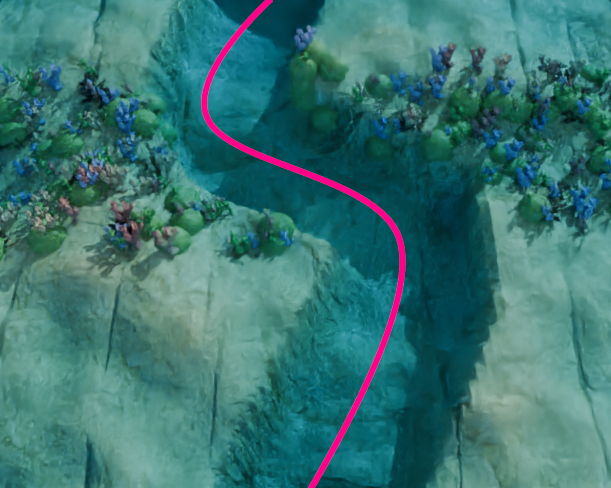
\includegraphics[width = 0.3 \linewidth]{Figures/Interactions/InteractionEdition1.png}
    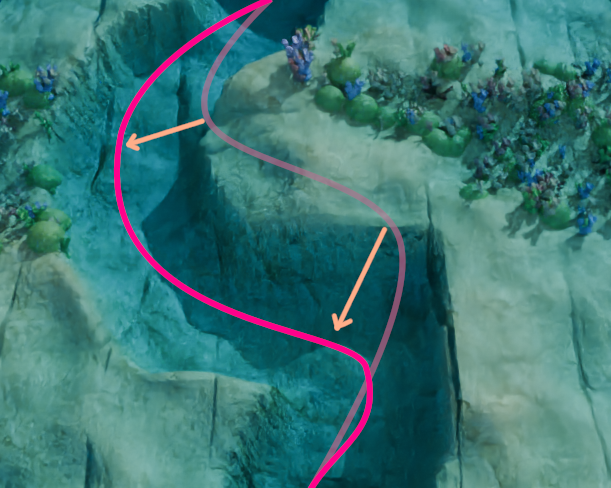
\includegraphics[width = 0.3 \linewidth]{Figures/Interactions/InteractionEdition2.png}
    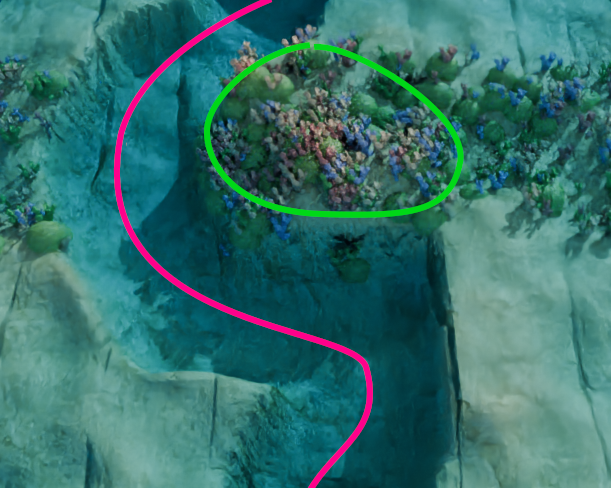
\includegraphics[width = 0.3 \linewidth]{Figures/Interactions/InteractionEdition3.png}
    \caption{Starting from a coral colony developed around a canyon (\textit{left}), the user edits the shape of the canyon, resulting in a different configuration of the scene, killing the corals that ends too deep in the water (\textit{center}) and the development and growth of new corals at the previous location of the canyon (\textit{right}). }
    \label{fig:semantic-representation_user-interaction}
\end{figure}

As long as a non-zero \gloss{FitnessFunc} is defined in the terrain, new \glosses{EnvObj} can be forced by the user at any point of the simulation. 

% \subsection{Guiding the simulation}
Control over the region of the terrain that should be updated can be given by adjusting all \glosses{FitnessFunc} through a scalar field $\influence: \R^2 \to \R $ such that the \gloss{FitnessFunc} $\fitnessFunc(\p)$ of any new \gloss{EnvObj} is evaluated as $\fitnessFunc^*(\p) = \influence{\p} \fitnessFunc(\p)$. This is especially useful in the planning of robotic simulations as we can first generate the overall shape of our terrain and secondly focus the generation process around the areas that may be visited by the robot, avoiding useless simulations and computer power. 
\cref{fig:semantic-representation_coral-colonization-scene} shows an example of colonization of the coral polyps that we limited manually into an annulus.
% \cref{fig:semantic-representation_focus-area-example} shows an example of colonization of the coral polyps that we limited manually.

% \begin{figure}
%     % \centering
%     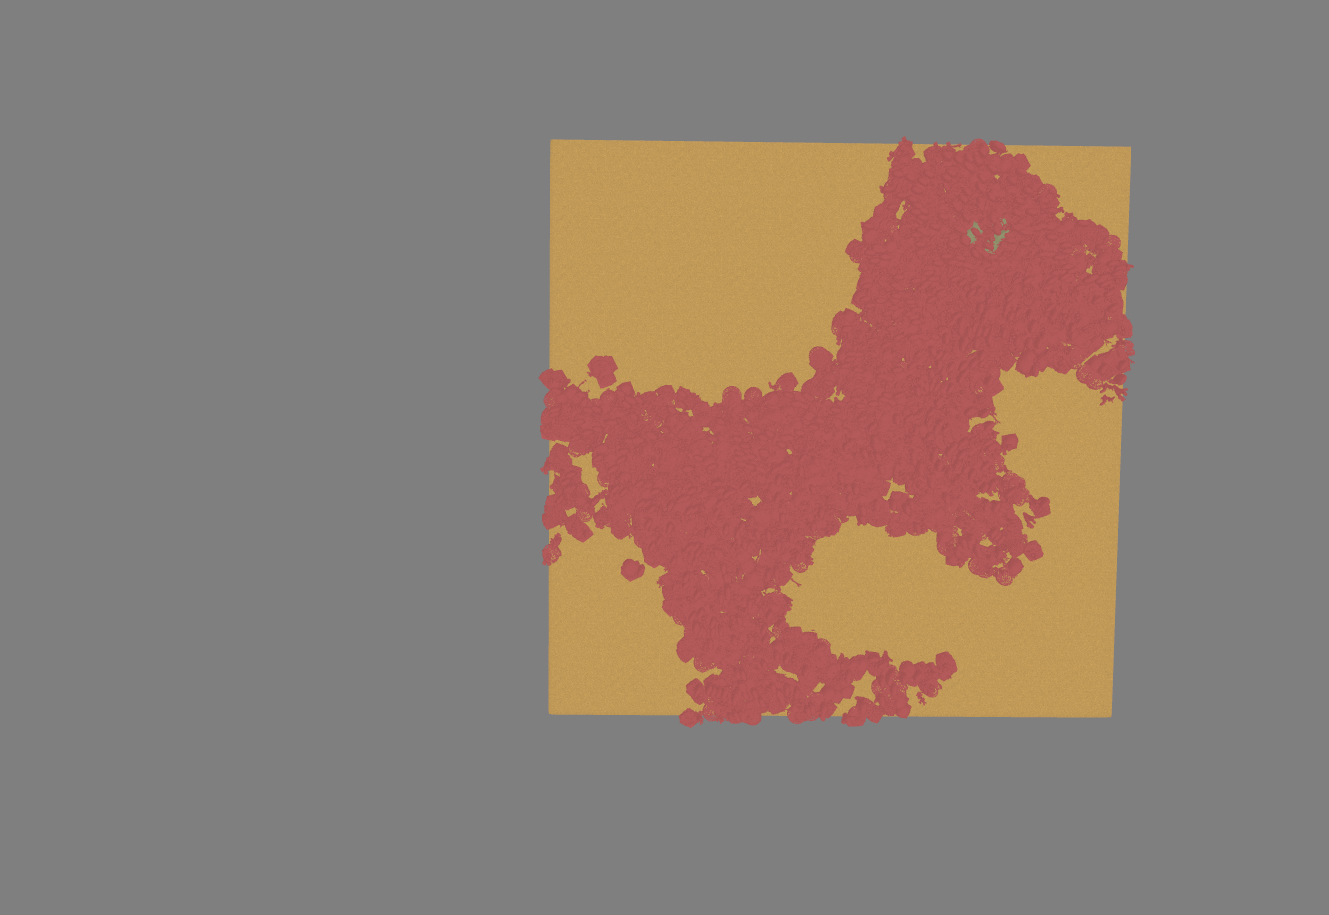
\includegraphics{Figures/UserControl/guidedGeneration1.png}
%     \caption{Controlling the generation area can produce a user-defined focused shape.}
%     \label{fig:semantic-representation_focus-area-example}
% \end{figure}

% - Changing the water currents

Our water current simulation is modeled as a simple vector field. As such, the user is able to interact with it at any moment of the simulation, allowing for the death of sensible \glosses{EnvObj} while it will guide the simulation into a new landscape. By modifying the water currents, the user also modifies the transport rate of \glosses{EnvMat} at this position. The modification of currents is given as a stroke, a parametric curve $\curve$ for which we evaluate $\Delta \Wuser(\p)$ just as for curved environment objects (\cref{sec:semantic-representation_water-currents}).

\subsection{Indirect interaction with \glosses{EnvObj}}
\label{sec:semantic-representation_events}
A configuration file can define in advance the different \glosses{GeoEvent} that should be triggered during the simulation. This can be useful to generate landscapes that are close to some existing locations. 
Multiple \glosses{GeoEvent} can be triggered either as sudden or continuous environmental changes. These changes play a huge role in the morphology of landscapes.
We define \glosses{GeoEvent} with a starting point and an ending point, such that at any time of the simulation we can compute the progress of the \gloss{GeoEvent} as $\tEvent \in [0, 1]$.

Water level changes are important \glosses{GeoEvent} that shape the underwater landscapes. As previously submerged \glosses{EnvObj} get elevated above water level, flora and fauna terrain features dry and die. Deprived from the living part of the features, everything is more affected by terrestrial erosion. By updating the value of the depth $\depth$ evaluated in the \glosses{FitnessFunc}, any \gloss{EnvObj} that is sensible to the depth will be impacted automatically, that may be causing death (\cref{fig:semantic-representation_water-event}). The modification of the water level is defined as 
\begin{align*}
    \depth(\p) = \depth_0(\p) + \sum_{e \in \events} \Delta \depth_e \tEvent
\end{align*}
with $\Delta \depth_e$ the amount of water rising or lowering during an \gloss{GeoEvent}. We assumed a linear evolution of the water level during an \gloss{GeoEvent}. This allows to evaluate the depth at any point in space and in time.

\begin{figure}
    % \centering
    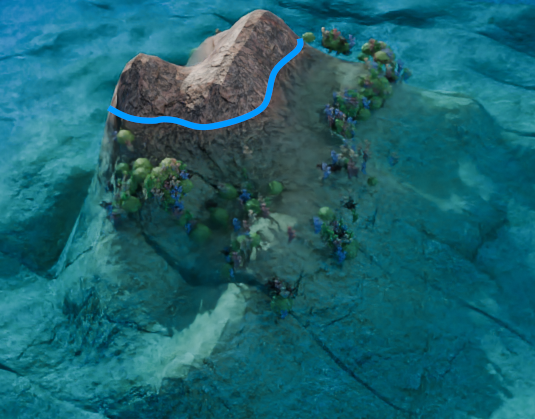
\includegraphics[width = 0.45 \linewidth]{Figures/Interactions/InteractionWater1.png}
    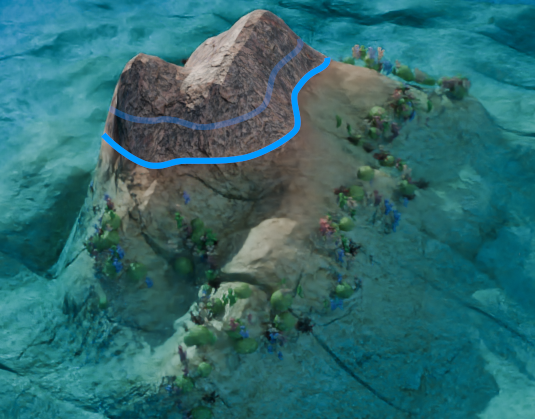
\includegraphics[width = 0.45 \linewidth]{Figures/Interactions/InteractionWater3.png}
    \caption{Lowering the water level by a few meters caused most of the coral objects to satisfy $\fitnessFunc \leq 0$, causing their death. Since the water level (blue) decrease slowly, new coral objects spawn progressively at a lower altitude.}
    \label{fig:semantic-representation_water-event}
\end{figure}

Subsidence and uplift are the main \glosses{GeoEvent} that create or destroy islands in the long term. These \glosses{GeoEvent} are simulated as a simple factor on the height field of the generated terrain (\cref{fig:semantic-representation_subsidence-event}). Subsidence is not always uniform in the terrain. As such, the user can provide a position $\q$ at which the subsidence is the strongest, the amount of subsidence applied $\Delta \height_e$ and a standard deviation $\std$ for which we can then compute at any point in space and time of the simulation the height of the terrain
\begin{align*}
    \height(\p) = \height_0(\p) \cdot \sum_{e \in \events}{G(\norm{\p - \q})} \Delta \height_e \tEvent 
\end{align*}
with $G(x)$ the Gaussian function
\begin{align*}
    G(x) = \exp \left(-\frac {x^{2}}{2 \std ^{2}}\right)
\end{align*}

\begin{figure}
    % \centering
    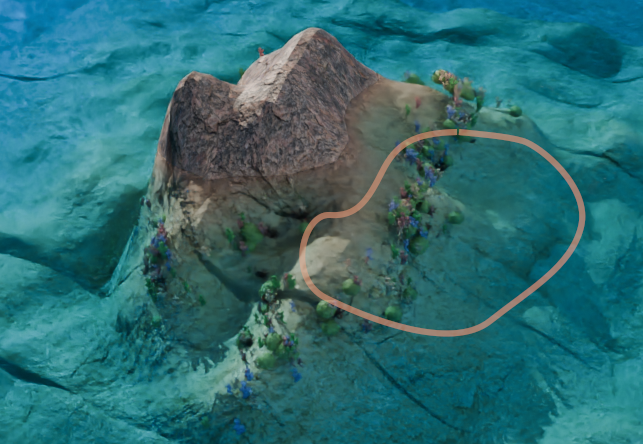
\includegraphics[width = 0.45 \linewidth]{Figures/Interactions/InteractionSubsidence1.png}
    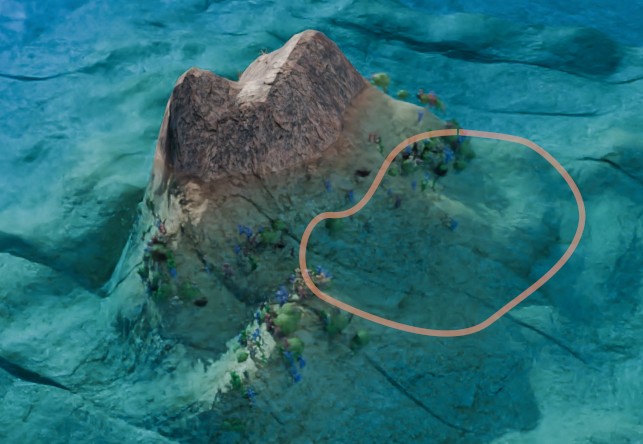
\includegraphics[width = 0.45 \linewidth]{Figures/Interactions/InteractionSubsidence2.png}
    \caption{Simulating subsidence on a part of the terrain (brown area) cause the depth value to change locally, resulting in the death of coral objects that find themselves too deep to survive. Here two subsidence \glosses{GeoEvent} are triggered in parallel. }
    \label{fig:semantic-representation_subsidence-event}
\end{figure}

Storms are factors of the geomorphology of coral reefs \cite{VilaConcejo2016, Oron2023} and coasts \cite{Dominguez2005, Cowart2010}. Due to the extreme wind and wave velocities coasts are highly eroded in a short time period and the more fragile corals near the water surface are broken, possibly causing breaches in the reefs and spreading polyps in the currents direction. While there are many factors at play to understand the apparition of storms and the hydrodynamics affecting it, we simplified the model of storms to the user as a single epicenter $\q$ with a wind velocity $\windVelocity$ and a standard deviation $\std$ representing the spread around the epicenter (\cref{fig:semantic-representation_storm-event}). The computation of water currents are then computed as 
\begin{align*}
    \Wuser(\p) = \Wuser^*(\p) + \sum_{e \in \events} {\windVelocity \frac{G(\norm{\p - \q}}{G(0)}}
\end{align*}
In this case, we did not include the linear factor $\tEvent$ as storms are usually conserving a constant force for the time of the few weeks or months of their occurrence. 

\begin{figure}
    % \centering
    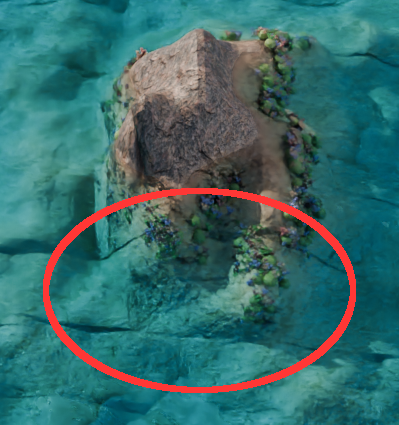
\includegraphics[width = 0.45 \linewidth]{Figures/Interactions/interactionStorm1.png}
    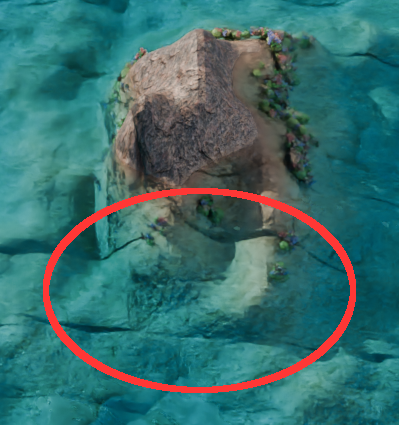
\includegraphics[width = 0.45 \linewidth]{Figures/Interactions/interactionStorm2.png}
    \caption{The result of a storm localized on one side of the island (red area) modifies the result of the evaluation of \glosses{EnvObj} around its epicenter for a short period of time. Most of the coral objects died from the \gloss{GeoEvent}, except few \glosses{EnvObj} less sensible to water currents strength. }
    \label{fig:semantic-representation_storm-event}
\end{figure}

% Just as for the rise and lowering of water level, the heat is modeled as a simple value of the environment. For shallow areas (<100m) we assume a linear relation between depth and temperature, and a constant value for the terrestrial environment. As such, we can model a heat wave by a change of the \glosses{EnvVal}. \Glosses{EnvObj} who are sensible to temperature may die instantly. The modification of the temperature is defined as 
% \begin{align*}
%     \temperature(\p) = T_0(\p) + \sum_{e \in \events} \Delta \temperature_e \tEvent + c \depth(\p)
% \end{align*}
with $\Delta \temperature_e$ the change of heat during an \gloss{GeoEvent}, $\temperature_0$ the temperature at the water surface, and $c$ a very small factor.

The framework can easily be extended as the \gloss{GeoEvent} system stays similar for all \glosses{GeoEvent}. Including higher level simulations in the \gloss{GeoEvent} system can be added, such as the simulation of tectonic activity, the use of fluid dynamics for tsunami \glosses{GeoEvent}, the integration of human activity, ...

\section{Results and discussion}
\label{sec:semantic-representation_results}
Our method provides a way to generate scenes at different scales. We demonstrate this capacity with the generation of a large scene of an island (\cref{fig:semantic-representation_teaser}) after what we focused the generation process in a canyon (\cref{fig:semantic-representation_canyon-scene}), then a small-scale visualization of coral colonies (\cref{fig:semantic-representation_coral-colonization-scene}).
In the examples, we rendered the \glosses{EnvObj} as a implicit tree or as individual meshes. The island, lagoons, reefs, canyons and sand ripples as implicit surfaces

% \subsection{Mid-scale}
% \label{sec:semantic-representation_mid-scale}
A canyon scene can be generated using our method. The water flow is affected by the curve of the canyon such that the currents are oriented in the direction of the curve's tangent.In this example, we force the position of arches to be inside the canyon. The arches deposits a material "rock deposit", which is the main element of the \gloss{FitnessFunc} of the Rock object. The "rock deposit" is slightly affected by water currents, but its mass make it highly affected by gravity. As such, rocks will spawn underneath arches. In reality, an arch is often created as part of a large coral boulder that sees the calcareous bottom part detached by the water currents, often resulting in an arch surrounded by big rocks and smaller rocks from the erosion of the first rocks.
As such, we define an \gloss{EnvObj} "Arch" with a \gloss{FitnessFunc} $\fitnessFunc_{arch}(\p) = 5 - d(canyon - \p) * \norm{\Water(\p)}$, an \gloss{EnvObj} "Rock" using $\fitnessFunc_{rock}(\p) = \material_{rock\_deposit}(\p)$ and Pebble using $\fitnessFunc_{pebble}(\p) = \material_{smaller\_rock\_deposit}(\p)$. Finally, sand ripples are simply described as curves appearing where there is a lot of sand available: $\fitnessFunc_{ripple}(\p) = \material_{sand}(\p)$.
Following these simple rules, \cref{fig:semantic-representation_canyon-scene} shows the emergence of details in the scene. 

% \subsection{Small-scale}
% \label{sec:semantic-representation_small-scale}
In this example we defined three different types of corals, coralA, coralB and coralC, to illustrate the possibility to model behaviours from the choice of \glosses{FitnessFunc}. Each of the coral types deposits a material "coral polyp" and "coral polyp A" ("coral polyp B" and "coral polyp C" respectively). By considering a \gloss{FitnessFunc} that minimize the ratio $\frac{\text{coral polyp}}{\text{coral polyp A}}$, we can see an emergent behavior of the three types of coral fighting for the space colonization.
\cref{fig:semantic-representation_coral-colonization-scene} shows the result of this simulation at three different interations. At the border between two colonies, none of the colonies make progression due to the amount of coral polyp specific from the other colony.

\begin{figure*}
    % \centering
    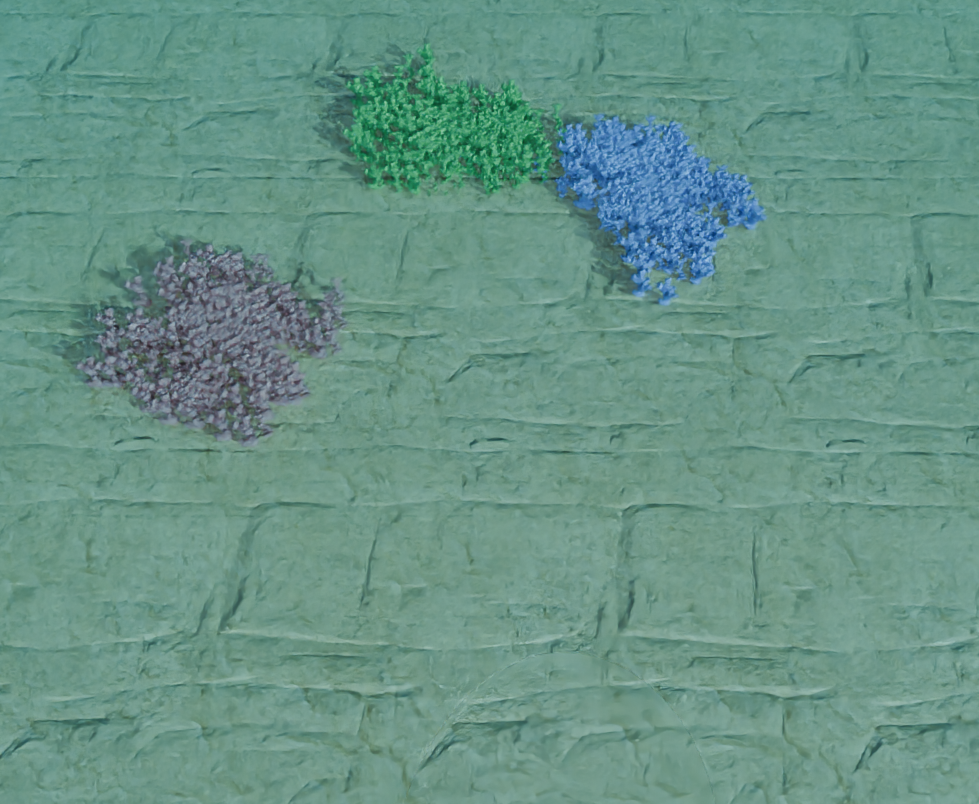
\includegraphics[width=0.24 \linewidth]{Figures/Colonization/col0.png}
    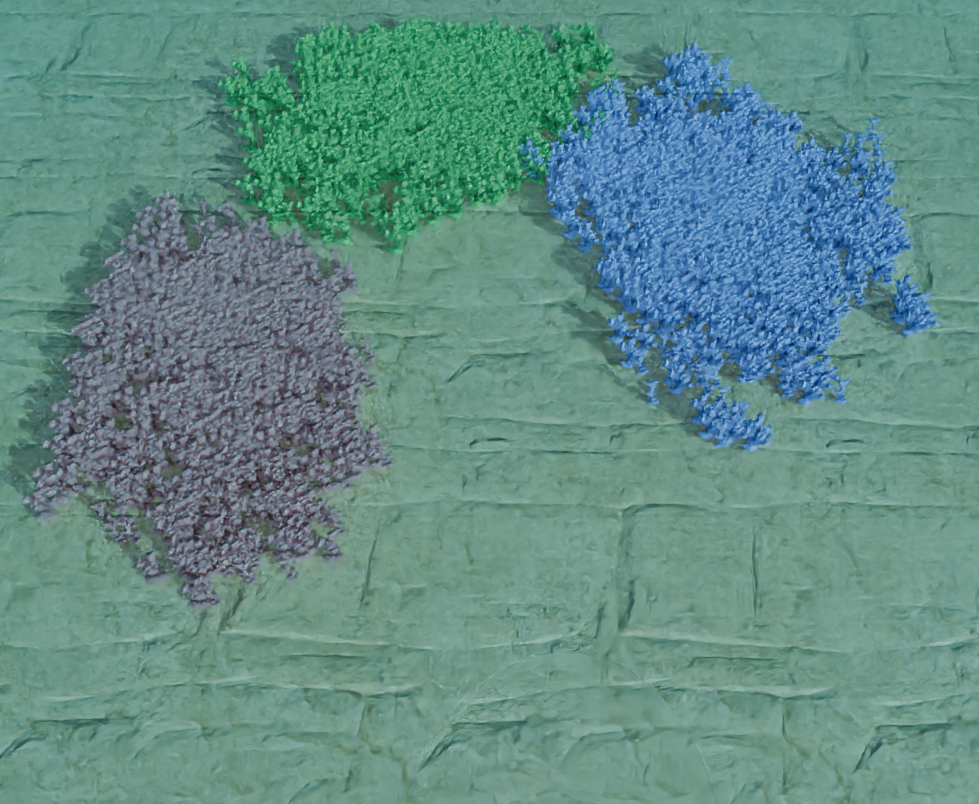
\includegraphics[width=0.24 \linewidth]{Figures/Colonization/col1.png}
    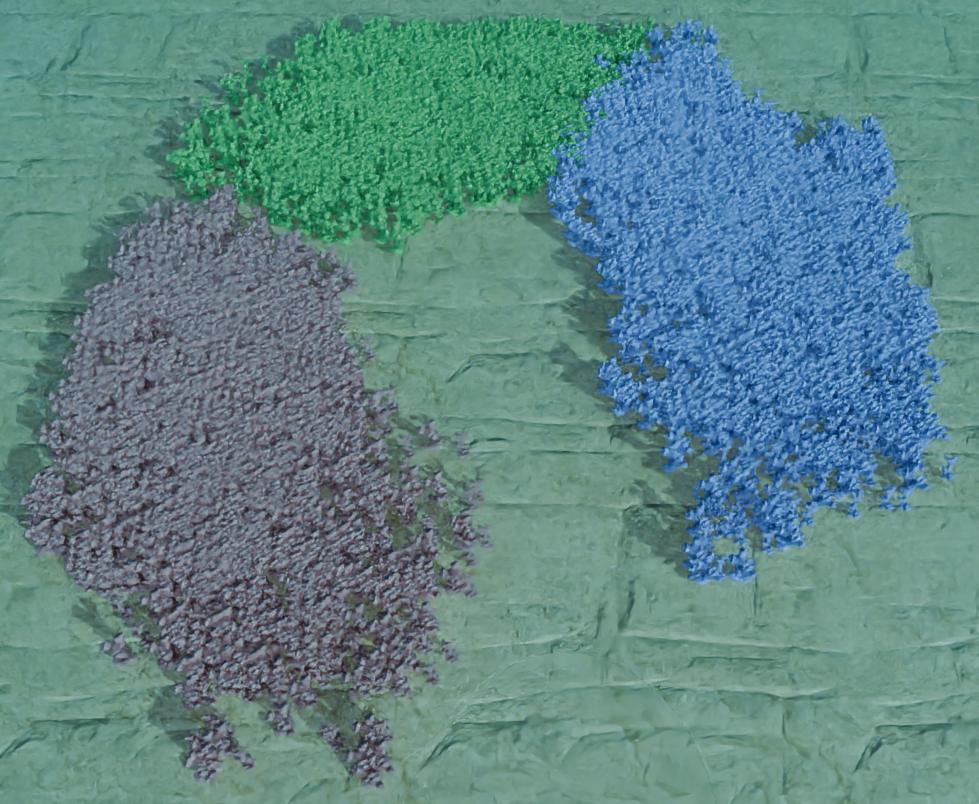
\includegraphics[width=0.24 \linewidth]{Figures/Colonization/col2.png}
    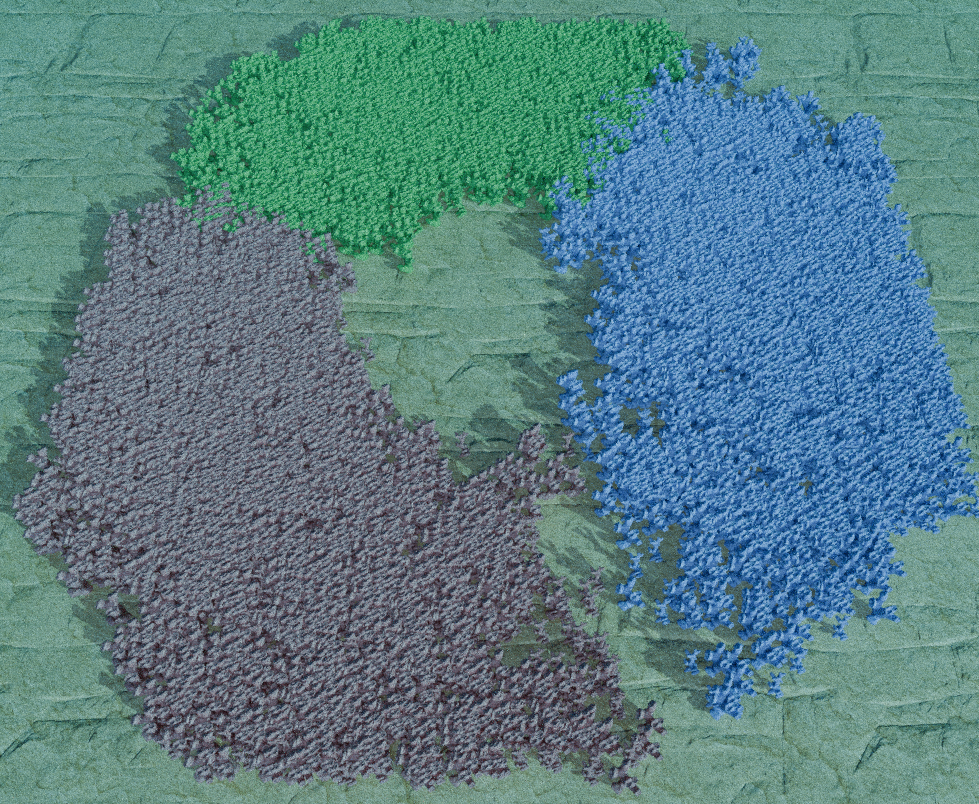
\includegraphics[width=0.24 \linewidth]{Figures/Colonization/col3.png}
    \caption{Three colonies of coral (red, blue, green) restricted to an annulus the middle section of the terrain fighting for the space.}
    \label{fig:semantic-representation_coral-colonization-scene}
\end{figure*}

\begin{figure*}
    % \centering
    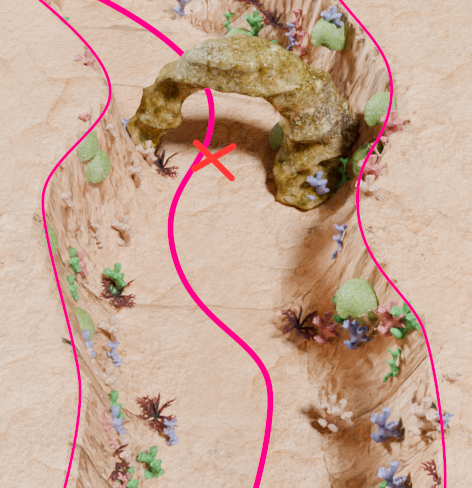
\includegraphics[width = 0.24 \linewidth]{Figures/Canyon/Canyon2.png}
    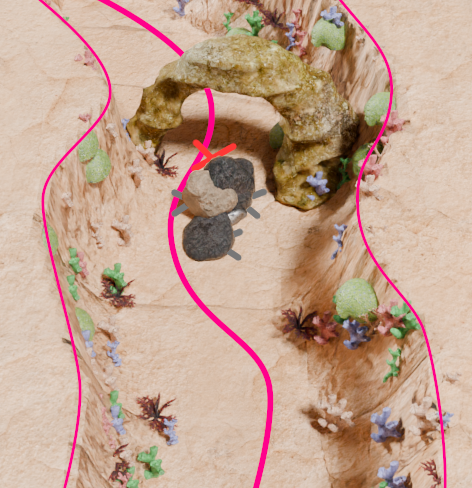
\includegraphics[width = 0.24 \linewidth]{Figures/Canyon/Canyon3.png}
    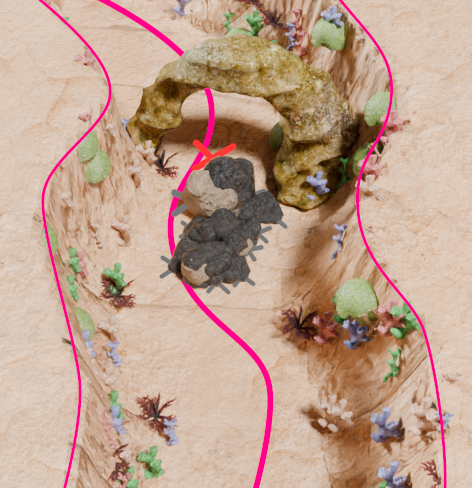
\includegraphics[width = 0.24 \linewidth]{Figures/Canyon/Canyon4.png}
    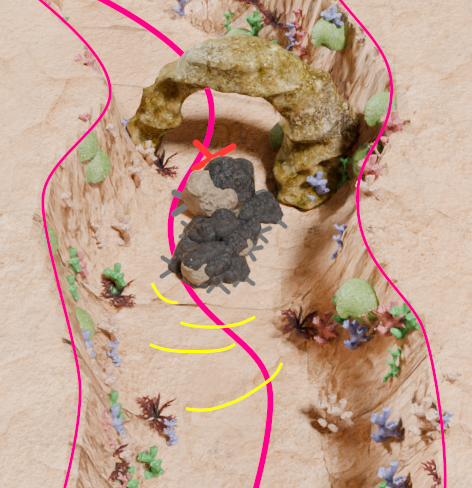
\includegraphics[width = 0.24 \linewidth]{Figures/Canyon/Canyon5.png}
    \caption{Evolution of a canyon scene at different iterations of the simulation. The apparition of an arch causes the spawning of rocks, pebbles, and finally some deposition of sand at the bottom of the canyon, spawning ripples. }
    \label{fig:semantic-representation_canyon-scene}
\end{figure*}


The proposed method aims to generate plausible landscapes using simplified versions of the evolution of an ecosystem and of the 3D representation. The biological realism of the result is highly correlated to the amount of simplification and assumptions, while the visual realism is completely dependent to the geometric functions used for the 3D modeling of the \glosses{EnvObj}. While proposing a flexible method that propose a generic approach for terrain generation, a close collaboration with fields experts and with graphists is needed to achieve optimal results.

Most simulation algorithm's quality depends on the size of the time step used, but with the introduction of a decay rate in the \glosses{EnvMat} properties, we limit the influence of time steps by considering that steady-state are reachable. The material deposition and absorption on punctual \glosses{EnvObj} can be seen as a Dirac function $\dirac$ centered at their position resulting in the advantage that material displacement function can use the definition of the diffusion equation instead of the advection-diffusion-reaction equation. This equation allowing us to evaluate the state of the material $\material$ without intermediate steps, but this is not applicable with curve- and region-based \glosses{EnvObj}. 

\section{Conclusion}
\label{sec:semantic-representation_conclusion}
We have proposed a method to generate terrains procedurally using sparse representations. This representation, the \glosses{EnvObj}, enables to introduce expert knowledge by the mean of the \glosses{FitnessFunc} that rule the \glosses{EnvObj} life cycle, but also to integrate the user in the loop during the generation process. We reduced the terrain resolution limitations by defining the environment objects as parametric features. Thanks to the sparse representation based on single points, curves and regions, we allow for direct manipulation of the \glosses{EnvObj} of the scene by the user which, thanks to the environment steady state consideration, also enables to include these interactions in the automatic simulation process.
Integrating environmental properties in the \gloss{FitnessFunc} of \glosses{EnvObj} allows the user to guide the generation through \glosses{GeoEvent}. Our method enables each \gloss{EnvObj} of the scene to influence the environment locally, reducing the need of computations while also retrieving \glosses{EnvVal} locally, which result in a parallelizable life-like simulation process. The genericity of the environment properties definitions should be sufficient for plausible generation of other landscape types as long as expert knowledge can be translated to \gloss{EnvObj}'s formalism.


We limited our work to the use of 2D scalar fields as they are more easily differentiable, interpretable and lighter than volumetric representations. However, future works include using 3D representations of the terrain and the environment to generate 3D terrains, including cavities, sub-terrestrial areas and the interior of coral structures. 
% The different possibilities to explore for this would be: the use of 3D particles to represent the state of the \glosses{EnvMat} in the environment, or voxel grids or flatten representation of the terrain's surface (but would not allow a different morphological shape than the height field...).

\begin{figure*}
    % \centering
    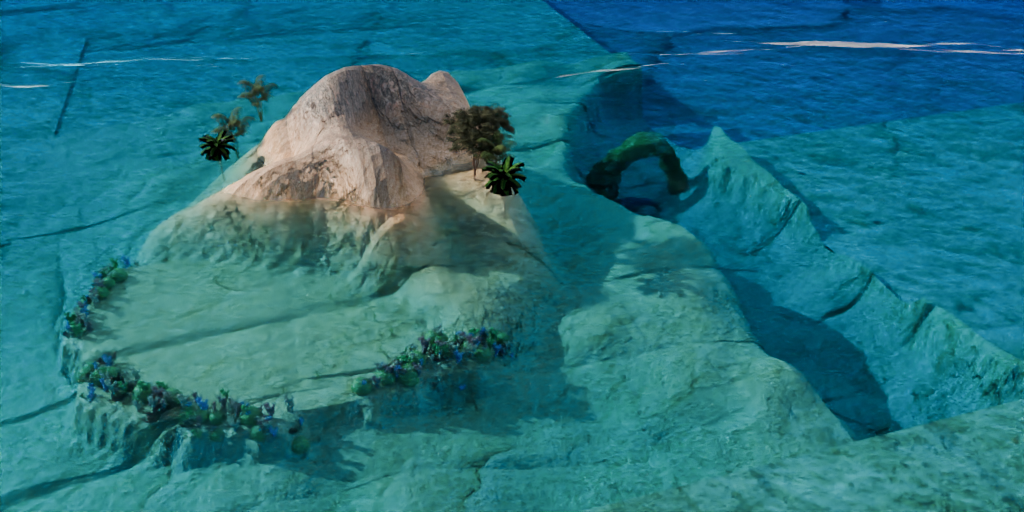
\includegraphics{Figures/CoralIsland/multiScene1 v2 final 1.png}
    \caption{A simple coral reef island is generated using an island, a lagoon, reefs coral polyps, beaches, trees and algae \glosses{EnvObj}. Trees appear on beaches and algae grow in the lagoon's sand. }
    \label{fig:semantic-representation_coral-island-scene}
\end{figure*}














% \section{Method}
% \label{sec:semantic-representation_method}
% The overall pipeline of the method is based on simple incremental generation like most rule-based systems. In this type of system, the final state is defined either by reaching equilibrium, or by verifying specific conditions, such as a maximum number of iterations. 
% We define our pipeline in three phases (\cref{fig:semantic-representation_pipeline}): the initialization phase that describe the generation and simulation rules, the iterative phase generating populating the terrain with our \glosses{EnvObj} and finally the output.


% \subsection{Pipeline overview}





















% \section{Expert knowledge integration}
% \label{sec:semantic-representation_biology}
%   The definition of the \glosses{FitnessFunc} of the \glosses{EnvObj} are inspired by the biological and geological factors that rule the evolution of underwater landscapes. The main factors are depth, light, water currents and biodiversity. External \glosses{GeoEvent} have direct and indirect repercussions on the biodiversity of underwater environments. Coral reef islands are complex bio systems in which fauna, flora and geology are mixed together. 

% \subsection{\Glosses{EnvObj} description}
% \label{sec:semantic-representation_represented-objects}
% We have represented with \glosses{EnvObj} some geologic features, animal features and flora features. The low island is most often raised in a circular shape as the process mainly appear around a hot spot under the ground. The evolution of an island into a coral reef island requires that the environmental conditions are sufficient for coral development: corals will grow slightly below the water surface as waves will break its growth and at a shallow depth (around 3m to 30m deep) in order for light to reach it. As coral grow and die, the skeleton is transformed into porous limestone, providing shelter to surrounding animals and reducing the impact of water erosion on the island. Corals drop polyps that are transported by the water flow and when they stick to a hard surface, as a rock or the reef itself, the coral may grow and colonize the area. As subsidence cause the island to lower, the living part of the coral reef keep growing toward light, which lead to a reef that is constantly close to the water level without reaching it due to wave erosion. The survival of reefs depends on the equilibrium between coral growth and and erosion. Eroded parts of the reef falling in the sheltered part of the reef accumulates, ending up by forming a lagoon. An island formed by a hot spot will inevitably subside in time, until it is completely flatten. As the coral reefs keep growing, only the lagoon remain, resulting in an atoll. \\
% In this work we we integrate the biological and geological knowledge in the \glosses{FitnessFunc} of the \glosses{EnvObj} we want to generate. We represent the islands as regions that can be appearing with a uniform distribution. From the formulation of the region description \eqref{eq:internal-energy-equation}, we mostly create circular islands. The coral features, \glosses{EnvObj} described as a single point, have a \gloss{FitnessFunc} that take into account the depth of the ground, the amount of sand, fresh water and polyps in their environment, as well as the strength of water currents. Each coral species have different living conditions, but we reduced our work to soft coral which are sensible to water strength and stony corals that are more resistant to erosion. Reefs are formed as coral's skeleton are transformed into calcareous stone, describing then as an \gloss{EnvObj} representing multiple others. 

% \subsection{Simplifications}
% \label{sec:semantic-representation_simplifications}
% The environmental factors simulated are greatly simplified as the real processes are in a very small time scale, that computer simulation are not able to simulate in interactive time. The use of \glosses{EnvObj} aim to represent a plausible results, while avoiding modeling the smaller scale \glosses{GeoEvent}. Examples of simplifications are the geometry and material of each \gloss{EnvObj}, which have an influence on the water currents through friction, the water currents represented as stationary flows, while the water flow dynamics are a complex system that may change completely at two different times of the day, the animal influence on the reefs that they transform by the ingestion and deposition of sediments, ...

%
%- What is semantic representation? \\
%** Linguistic definition + Image definition + Our definition \\
%- Why use semantic representation? \\
%** Sharing knowledge with biologists, geologists, etc. \\
%** Data from travel journals, labeled maps, ... \\
%- Advantages and disadvantages of semantic representation \\
%** Advantages: \\
%*** Interpretation \\
%*** User control \\
%*** 3D representation abstraction \\
%** Disadvantages: \\
%*** Need for expert knowledge (+ interdisciplinary communication issues) \\
%*** Necessary simplifications in physics / natural phenomena \\
%- 3D representation of semantic terrains \\
%** Possible combinations of methods (implicit functions + meshes)
%
%\section{Sparse terrain representation}
%- Landscape contains structures of very varying sizes: \\
%** Mountains covering several km² but rivers a few meters wide, for example \\
%- Proposal for sparse terrain representation \\
%** Definition of terrain elements as simple objects: environmental objects \\
%** Implicit geometry, offering 2D or 3D display \\
%** "Easy" LOD possibility \\
%- Iterative method for generating sparse terrain \\
%** Reduce computation time from $O(n^2)$ to $O(n)$ by using the environment as a proxy \\
%** Method based on material deposition \\
%** Iterative stochastic process
%
%\section{Environmental objects}
%- Symbolism of the environmental object \\
%- Reference to "Environmental Objects" \\
%- Comparison to biotopes
%
%\subsubsection{Definition}
%- Skeleton \\
%- Parametric shape \\
%- Living conditions
%
%\subsubsection{Implementation}
%- Instantiation of objects \\
%** Definition of the skeleton \\
%*** Points, curves, regions \\
%*** Use of Snake \\
%** Definition of geometry \\
%- Modifications to the environment \\
%- ...
%
%% \chapter{Snake - Active Contour Model}

We want to symbolize a dead coral area as a \gloss{EnvObj} "reef." To do this, the coral objects continuously deposit a quantity of "dead coral" material. This material, stored in a discrete scalar field, contains high intensities where a reef should supposedly exist. 
We need to draw a curve to represent this new object. The constraints of this curve are that it must pass through the points of highest intensity while maintaining a given length.

The Snake algorithm, or Active Contour Model, approaches this application. The algorithm proposes to give an energy to the curve, which then tries to minimize it through gradient descent.

The energy, in the initial paper, is defined by
\begin{align}
    \Esnake^{*} = \int \limits _{0}^{1} { \Esnake(\mathbf {v} (s))\,ds } = \int \limits _{0}^{1} { \Einternal (\mathbf {v} (s)) + \Eexternal (\mathbf {v} (s)) } \,ds
\end{align}

The internal energy represents the properties of the curve while the external energy represents properties of the field it lies in. In the original paper they are described as: 
\begin{align}
    \Einternal &= \alpha \Econt + \beta \Ecurv \\
    \Eexternal &= \gamma \Eimage
\end{align}

The continuity cost $\Econt$, originally defined as the minimization of the spacing between the points $\left\|{\frac {d{\bar {v}}}{ds}}(s)\right\| ^{2}$, does not make much sense in the discrete form of the algorithm. In its discrete form, we seek to maintain a regular interval between the points by applying $\Econt = \left(\tilde{d} - \left\|p_i - p_{i-1} \right\| \right)^2$ with $\tilde{d}$ being the average distance between each point.

The curvature cost $\Ecurv$ seeks to minimize the oscillations of the curve and can thus be defined as the squared second derivative $\left\|{\frac {d^{2}{\bar {v}}}{ds^{2}}}(s)\right\| ^{2}$.

The discrete form $\Ecurv^{*} = \left\| p_{i-1} - 2 p_i + p_{i+1} \right\| ^2$ is not necessary with splines, due to their closed form.

The image cost $\Eimage$ tries to attract the points of the curve to a local maximum of the image gradient. It is defined as $\Eimage = - \left\| \nabla I \right\| $.

We want to see our curve maintain a given length $L$. We then modify the formulation of the continuity cost to become $\Econt = \left(\tilde{l} - \left\|p_i - p_{p-1} \right\| \right)^2$ with $l = \frac{L}{n - 1}$, knowing $n$ is the number of vertices of the curve. Additionally, we want a curve that follows points of high intensity rather than the gradient, which leads to modifying the image cost $\Eimage = -I$.

The calculation of the gradient $\nabla \Esnake$ remains trivial in parts:
\begin{align}
    \frac{\partial \Eimage}{\partial p_i} &= - \nabla I(p_i) \\
    \frac{\partial \Ecurv^{*}}{\partial p_i} &= -\frac{2 \left( p_{i-1} - 2 p_i + p_{i+1} \right) }{ \left\| p_{i-1} - 2 p_i + p_{i+1} \right\| } \\
    \frac{\partial \Econt^{*}}{\partial p_i} &= 2 \left(l - \left\|p_i - p_{i-1} \right\| \right) \cdot \frac{p_i - p_{i-1}}{ \left\| p_i - p_{i-1} \right\| }
\end{align}

We then have
\begin{align}
    \Esnake &= \alpha \left(l - \left\|p_i - p_{i-1} \right\| \right)^2 + \beta \left\| p_{i-1} - 2 p_i + p_{i+1} \right\| ^2 - \gamma I \\
    \nabla \Esnake &= 2 \alpha \left(l - \left\|p_i - p_{i-1} \right\| \right) \cdot \frac{p_i - p_{i-1}}{ \left\| p_i - p_{i-1} \right\| } - \beta \frac{2 \left( p_{i-1} - 2 p_i + p_{i+1} \right) }{ \left\| p_{i-1} - 2 p_i + p_{i+1} \right\| } - \gamma \nabla I(p_i)
\end{align}

It should be noted that the calculation of $\Econt^{*}$ uses the distance $\left\|p_i - p_{i - 1} \right\|$. For $i = 0$, the distance $\left\| p_i - p_{i + 1} \right\|$ is used.

If all the points of the curve are at a distance greater than $l$, the optimization will push each of these points to get closer to its predecessor. Point $p_0$, itself, will move very little, so the entire curve aligns towards point $p_0$. By using the distance to the successor $\left\| p_i - p_{i+1} \right\|$, the curve moves towards point $p_N$.
It is then possible to converge towards the median point by alternating the use of the distance with the predecessor and with the successor, at the cost of slower convergence.

The active contour model algorithm is highly sensitive to the initial curve placement. In cases where a portion of the curve is in an area with a very low gradient on $\Eimage$, the vertices of the curve will simply optimize $\Einternal$, resulting in a straight segment in a low-intensity area, while the rest of the curve optimizes correctly.

To mitigate this problem, we propose adapting the Snake algorithm into Caterpillar: throughout the gradient descent, the target length $L$ is artificially reduced and then increased. In this way, a portion of the curve blocked in a region without possible optimization on external energy will be attracted by the optimized curve until it falls on a strong gradient. The dead portion can take the place of optimized vertices. By returning the target length $L$ to its initial value, the optimization continues with fewer vertices in the dead zone. Repeating this process gradually brings all points into an optimizable area. However, a too-rapid change in the target length can prevent the vertices from optimizing $\Eexternal$ by amplifying $\Einternal$ too much. Additionally, this algorithm can lead to numerical errors and slower convergence.

%
%\subsection{Communication between objects}
%- Comparisons with reality \\
%** No direct communication between elements \\
%- ...
%
%\subsubsection{Interactions through the environment}
%- Modifications to the environment \\
%** Absorption \\
%** Deposition \\
%** Modification of currents \\
%- Impact of the environment on objects \\
%- ...
%
%\subsubsection{Lifecycle of environmental objects}
%- ...
%
%\section{Results}
%- ...


%\subsection{Implemented tools}
%- Cost function parser \\
%- ...

%\section{Other attempts}
%\subsection{Direct interactions}
%\subsubsection{Graph generation}
%\subsubsection{Delaunay triangulation}


%
%\section{Continuous erosion}
%[POSSIBLY TO BE MOVED TO EROSION] \\
%- ...
%
%\subsection{Problem description}
%- Erosion process is a dynamic system \\
%- Very large number of variables \\
%- Impossible to simulate at different time steps and/or different scales/resolutions
%
%\subsection{Proposed solutions}
%- ...
%
%\subsubsection{Lifecycle of environmental objects}
%- ...
%
%\subsubsection{Use of deep learning}
%- ...




%\chapter{Influence sur la génération}
\label{chap:influence-on-env-objects}
\minitoc


\section{Introduction}
\label{sec:influence-on-env-objects_introduction}
This document aims to formalize a terrain generation method developed during my thesis.

The main issue this method seeks to address is the difficulty for a user to describe the environments they want to generate. By proposing a hierarchical structure in the description of elements to define, the environments exhibit adaptive representation granularity, catering both to the user's needs and hardware capabilities.

The key element of the method is the "biotope," defined as "a habitat defined by relatively uniform physical and chemical characteristics." (Source: Wikipedia)

In this context, we define the characteristics of a geographical region as well as the sub-biomes included within it.

Although this method was conceived with the aim of generating underwater environments, many examples given in this document will use elements present in surface environments, purely for simplification purposes.

\section{Glossary}
\label{sec:influence-on-env-objects_glossary}
Initially, this document will present definitions of various terms used in the description of the method. By doing so, we hope to eliminate any ambiguity in the upcoming explanations. Definitions may appear in certain sections of this document if deemed too specific.

\textbf{Biotope}: The main element of the method used. The biotope (or, as I might often write, the biome) is a geographical region defined by topographic and geomorphological characteristics. The notion of biotope used does not distinguish between different scales (the biosphere and the ecosystem of a rock are represented uniformly), nor does it distinguish between living and mineral elements. The biotope is represented in two different ways in the terrain generation process: the model and the instance.

\textbf{Model (of biotope)}: The model (or biotope model, if the context requires) is a biological description of the geographical area. It remains an abstract, or literary, form of the biotope. It is defined by a list of characteristics related to topography (description of the relief, description of the shape of the region) and geology (type of soil, for example). One can also list the sub-biomes that compose it, specifying the quantity, proportion, chances of appearance, etc., of each sub-biome. This form is the user input into the system, but during the terrain generation process, the model's role is to create instances of itself to concretize the structure to be generated. In the document illustrations, if a model is represented in a graph, it will be symbolized by its name in quotation marks (e.g., "Forest," "Lagoon").

\textbf{Instance (of biotope)}: The instance is the concrete form of the model. Unlike the model, the instance takes place in space with fixed characteristics (unlike the probabilistic characteristics of the model). Through generation rules and living conditions defined by the user and the system, the biotope instance has a geometric shape and neighboring relationships with other instances. An instance, like its original model, consists of sub-biomes. The instance remains linked to its original model. To distinguish the instance from the model in the document illustrations, if represented in a graph, the instance will be symbolized by the model's name followed by a hash and an instance number (e.g., Forest \#1, Lagoon \#28).

\textbf{Generation Rule}: Generation rules represent a list of obligations or prohibitions, including living conditions and adjacency rules.

\textbf{Living Condition}: In our definition, a biotope can only exist under certain environmental conditions in a specific place. The conditions can be multiple and will be listed in a subsequent chapter of this document. Vegetative elements, for example, have strong constraints in terms of sunlight exposure, the "snow" biotope requires a low temperature condition, and some biotopes like sand cannot exist on steep terrain. Living conditions are therefore important properties to express in biotope models. These conditions can be expressed probabilistically.

\textbf{Adjacency Rules}: Adjacency rules define how biotope instances can be arranged. There are three types of rules to express adjacency between two biotopes: prohibition, possibility, and obligation. Two models linked by an adjacency prohibition cannot generate instances with a common border. Conversely, a model linked to another by an obligation constraint can only generate an instance if it shares a border with an instance of the linked model. The possibility constraint is the default, where the instance is indifferent to the presence or absence of a common border. It is conceivable that the notion of "possibility" could be associated with a probability in the future, allowing for example, a lake to often be adjacent to an urban area, but an urban area to rarely be near a desert. For now, adjacency rules are bilateral: a rule that applies from biotope A to biotope B also applies from B to A. In the rest of the document, adjacency rules will mainly be represented by graphs (undirected) with the nodes as the models to be generated, solid edges representing the possibility of adjacency, dotted edges symbolizing an adjacency obligation (rarely used), and the lack of an edge indicating an adjacency prohibition.

\textbf{Adjacency Graph}: The adjacency graph, although similar to the representation of adjacency rules, this time represents the concrete topological adjacency between the generated instances (not the models). The adjacency graph consists of nodes representing each instance generated by the models and the edges representing the existence of a common border. Edges can only be present if the two biotope instances see their model linked either by an obligation or possibility of adjacency constraint. By definition, this graph must be planar. In this document, adjacency graphs will therefore be represented by graphs where the nodes are biotope instances (following the instance graphic convention), and an edge represents a topological adjacency.

\textbf{Region (of biotope)}: The region is the space occupied in a geometric sense by a biotope instance once represented in space. Among the important properties, one can note that a region has a shape and an area.

\textbf{Boundaries}: The boundary is the geometric adjacency of two regions representing biotope instances.

\textbf{Adjacent Regions}: Two regions are adjacent if they share a common edge. In a successful generation, a region shares a common boundary with regions represented by instances linked to the current region instance in the adjacency graph. We can then distinguish three types of connections between instances: correctly adjacent instances are linked in the adjacency graph and are adjacent regions, over-adjacent instances are not linked in the adjacency graph and are adjacent regions, and under-adjacent instances are linked in the adjacency graph and are not adjacent regions. The latter two types are maladjacencies.

\textbf{Biotope Characteristics}: Biotopes possess characteristics common at all scales, whether they represent geological or biological elements. The characteristics are defined in the models in probabilistic forms. Instances inherit a unique and fixed value for each characteristic from the original model. The characteristics notably define the shape the generated region will take, the relief, etc.

\textbf{Sub-biotope}: Each biotope can include one or more sub-biomes. This is how an environment can be defined on the scale of a planet as well as on the scale of a rock. The biotope specifies the number of instances to generate for each sub-biome, or the proportion of the surface to cover. The parent biotope provides an approximate description of its environment, but with each sub-biome, the description is refined.

\textbf{Recursive Tree}: The proposed method has a strong recursive nature through its representation in biotopes and sub-biomes. The biotope construction tree is thus a recursive tree of biotopes composed at the root of a biotope to be generated and whose nodes (and leaves) represent sub-biomes. The parent-child relationship defines the inclusion of the child among the sub-biomes of the parent node. The tree describing a biotope can then be reused to describe a larger biotope, up to a planetary scale or larger.

\textbf{User Action}: The user plays an important role in the terrain generation process. By user action, we mean any action performed during the process. User actions are applied to biotope instances: adding, replacing, or deleting an instance, or modifying the characteristics and living conditions of an instance.

\textbf{Primitives}: Primitives are simple geometric representations that can be combined to represent more complex structures. Among these, we can notably find: the point, the curve, the sphere, and the 3D model.

\section{Environment description}
\label{sec:influence-on-env-objects_environment-description}
In this method, an environment is defined by a biotope model for which characteristics such as the general shape of its region, the biotope's relief, or the representative primitive of the biotope are specified, as well as living conditions such as altitude, temperature, and necessary luminosity for its survival. These characteristics are uniform across the entire biotope region; the only way to vary them is to add sub-biomes in the definition, which will take the form of sub-regions of the parent. Sub-biomes have the same types of characteristics and living conditions, which they can define in their own way, as well as their own sub-biomes.

Thus, the environment description is carried out recursively until the level of detail is sufficient for the modeler.

A biotope model can be the sub-biome of several different biotope models, offering the possibility to define complex environments quickly.

\subsection{Biotope characteristics}
The biotope model allows the user to describe the biotope's appearance to be generated. This description is probabilistic, and instances derived from the model each define a unique value for each characteristic respecting the probability law described by the model. The list of characteristics includes:
\begin{itemize}
	\item Region size: This represents the area of the surface (without considering relief) that the region occupies in space.
	\item Altitude (min and max): These two characteristics represent the altitudes the biotope can reach.
	\item Relief (frequency and amplitude): These characteristics describe the terrain's gradient. High relief amplitude symbolizes significant disturbances on the ground, unlike low amplitude, which
	
	indicates the ground is relatively flat.
	\item Primitive (type, dimension, position): The primitive determines the basic element represented by the biotope.
	\item Shape: The biotope region's shape in space.
\end{itemize}

To facilitate the user's work, default values are proposed for each biotope, respecting each type of primitive.

\subsection{Living conditions}
The living conditions of a biotope define the specific properties necessary for the biotope to survive. To be viable, the biotope must respect these conditions. These properties may relate to the following conditions:
\begin{itemize}
	\item Luminosity (min and max)
	\item Temperature (min and max)
	\item Soil type
	\item Exposure (direction, minimum and maximum angle)
\end{itemize}

Like characteristics, default living conditions are proposed to the user.

\subsection{Adjacency rules}
Three types of rules express adjacency between two biotopes: prohibition, possibility, and obligation. These rules define how biotope instances can be arranged spatially.

\begin{itemize}
	\item Prohibition: Two models linked by an adjacency prohibition cannot generate instances with a common border.
	\item Possibility: Instances can be adjacent, but it is not required.
	\item Obligation: Instances must share a common border.
\end{itemize}

\section{Generation process}
\label{sec:influence-on-env-objects_generation-process}
The terrain generation process involves creating instances from biotope models while respecting their characteristics, living conditions, and adjacency rules. This section details the steps of the process.

\subsection{Instance creation}
Each biotope model creates instances with fixed values for each characteristic derived from the probabilistic descriptions in the model. These instances are then positioned in space according to their characteristics and living conditions.

\subsection{Placement and adjustment}
Instances are placed in the environment, respecting their adjacency rules. If instances violate adjacency constraints, adjustments are made to either reposition instances or modify their characteristics within acceptable limits.

\subsection{User interaction}
Users can intervene in the generation process by adding, replacing, or deleting instances, as well as modifying instance characteristics and living conditions. These actions allow for fine-tuning the generated environment.

\subsection{Validation and refinement}
The final step involves validating the generated environment by checking for over- or under-adjacencies and making necessary refinements to ensure all instances adhere to their constraints and living conditions.

\section{Conclusion}
\label{sec:influence-on-env-objects_conclusion}
This method provides a structured approach to terrain generation by leveraging biotopes and their hierarchical organization. By defining biotopes probabilistically and respecting adjacency rules and living conditions, it is possible to generate diverse and realistic environments with varying levels of detail.

Future work may include refining probabilistic models for characteristics and adjacency rules, as well as exploring the use of probabilistic adjacency possibilities to further enhance the flexibility and realism of generated terrains.
%- ...
%
%\section{Biotope generation}
%- ...
%
%\subsection{Definition}
%- ...
%
%\subsubsection{Recursion}
%- ...
%
%\subsubsection{Voronoi diagram}
%- ...
%
%\subsubsection{Communication between biotopes}
%- ...
